\NumberThisInToc
\chapter{MUTE, un éditeur de texte web collaboratif P2P temps réel chiffré de bout en bout}
\minitoc
\label{chap:mute}

Les systèmes collaboratifs temps réels permettent à plusieurs utilisateur-rices de réaliser une tâche de manière coopérative.
Ils permettent aux utilisateur-rices de consulter le contenu actuel, de le modifier et d'observer en direct les modifications effectuées par les autres collaborateur-rices.
L'observation en temps réel des modifications des autres favorise une réflexion de groupe et permet une répartition efficace des tâches.
L'utilisation des systèmes collaboratifs se traduit alors par une augmentation de la qualité du résultat produit \cite{2004-empirical-study-collaborative-writing, 2005-internet-encyclopaedias-head-to-head}.

Plusieurs outils d'édition collaborative centralisés basés sur l'approche \ac{OT} \cite{1989-grove-ellis-gibbs} ont permis de populariser l'édition collaborative temps réel de texte \cite{gdocs, etherpad}.
Ces approchent souffrent néanmoins de leur architecture centralisée.
Notamment, ces solutions rencontrent des difficultés à passer à l'échelle \cite{2015-cope-delay-collaborative-note-taking-ignat, 2016-performance-collaborative-editors-dang-ignat} et posent des problèmes de confidentialité \cite{prism-washington-post, prism-guardian}.

L'approche \ac{CRDT} offre une meilleure capacité de passage à l'échelle et est compatible avec une architecture \ac{P2P} \cite{2011-evaluation-crdts-ahmed-nacer}.
Ainsi, de nombreux travaux \cite{Nedelec2016CRATE, peerpad, serenity-notes} ont été entrepris pour proposer une alternative distribuée répondant aux limites des éditeurs collaboratifs centralisés.
De manière plus globale, ces travaux s'inscrivent dans le nouveau paradigme d'application des \emph{Local-First Softwares} \cite{localfirstsoftware2019, pushpin2020}.
Ce paradigme vise le développement d'applications collaboratives, \ac{P2P}, pérennes et rendant la souveraineté de leurs données aux utilisateurs.\\

\mnnote{TODO: Serait intéressant d'ajouter une catégorisation des éditeurs collaboratifs en fonction de leurs caractéristiques (décentralisé vs. p2p, pas de chiffrement vs. chiffrement serveur vs. chiffrement de bout en bout, OT vs CRDT vs mécanisme de résolution de conflits custom...) pour mettre en avant le caractère unique de MUTE}

De manière semblable, l'équipe Coast conçoit depuis plusieurs années des applications avec ces mêmes objectifs et étudient les problématiques de recherche liées.
Elle développe \acf{MUTE} \cite{MUTE2017}\footnote{Disponible à l'adresse : \url{https://mutehost.loria.fr}}\footnote{Code source disponible à l'adresse suivante : \url{https://github.com/coast-team/mute}}, un éditeur collaboratif \ac{P2P} temps réel chiffré de bout en bout.
\ac{MUTE} sert de plateforme d'expérimentation et de démonstration pour les travaux de l'équipe.

Ainsi, nous avons contribué à son développement dans le cadre de cette thèse.
Notamment, nous avons participé à :
\begin{enumerate}
  \item L'implémentation des \acp{CRDT} LogootSplit \cite{2013-logootsplit} et RenamableLogootSplit \cite{2022-rls-tpds-nicolas} pour représenter le document texte.
  \item L'implémentation de leur modèle de livraison de livraison respectifs.
  \item L'implémentation d'un protocole d'appartenance au réseau, SWIM \cite{swim2002}.
\end{enumerate}

Dans ce chapitre, nous commençons par présenter le projet \ac{MUTE} : ses objectifs, ses fonctionnalités et son architecture système et logicielle.
Puis nous détaillons ses différentes couches logicielles : leur rôle, l'approche choisie pour leur implémentation et finalement leurs limites actuelles.
Au cours de cette description, nous mettons l'emphase sur les composants auxquelles nous avons contribué, \ie les sous-sections \ref{sec:mute-crdts}, \ref{sec:mute-delivery-model} et \ref{sec:mute-membership-protocol}.Les systèmes collaboratifs temps réels permettent à plusieurs utilisateur-rices de réaliser une tâche de manière coopérative.
Ils permettent aux utilisateur-rices de consulter le contenu actuel, de le modifier et d'observer en direct les modifications effectuées par les autres collaborateur-rices.
L'observation en temps réel des modifications des autres favorise une réflexion de groupe et permet une répartition efficace des tâches.
L'utilisation des systèmes collaboratifs se traduit alors par une augmentation de la qualité du résultat produit \cite{2004-empirical-study-collaborative-writing, 2005-internet-encyclopaedias-head-to-head}.

Plusieurs outils d'édition collaborative centralisés basés sur l'approche \ac{OT} \cite{1989-grove-ellis-gibbs} ont permis de populariser l'édition collaborative temps réel de texte \cite{gdocs, etherpad}.
Ces approchent souffrent néanmoins de leur architecture centralisée.
Notamment, ces solutions rencontrent des difficultés à passer à l'échelle \cite{2015-cope-delay-collaborative-note-taking-ignat, 2016-performance-collaborative-editors-dang-ignat} et posent des problèmes de confidentialité \cite{prism-washington-post, prism-guardian}.

L'approche \ac{CRDT} offre une meilleure capacité de passage à l'échelle et est compatible avec une architecture \ac{P2P} \cite{2011-evaluation-crdts-ahmed-nacer}.
Ainsi, de nombreux travaux \cite{Nedelec2016CRATE, peerpad, serenity-notes} ont été entrepris pour proposer une alternative distribuée répondant aux limites des éditeurs collaboratifs centralisés.
De manière plus globale, ces travaux s'inscrivent dans le nouveau paradigme d'application des \emph{Local-First Softwares} \cite{localfirstsoftware2019, pushpin2020}.
Ce paradigme vise le développement d'applications collaboratives, \ac{P2P}, pérennes et rendant la souveraineté de leurs données aux utilisateurs.\\

\mnnote{TODO: Serait intéressant d'ajouter une catégorisation des éditeurs collaboratifs en fonction de leurs caractéristiques (décentralisé vs. p2p, pas de chiffrement vs. chiffrement serveur vs. chiffrement de bout en bout, OT vs CRDT vs mécanisme de résolution de conflits custom...) pour mettre en avant le caractère unique de MUTE}

De manière semblable, l'équipe Coast conçoit depuis plusieurs années des applications avec ces mêmes objectifs et étudient les problématiques de recherche liées.
Elle développe \acf{MUTE} \cite{MUTE2017}\footnote{Disponible à l'adresse : \url{https://mutehost.loria.fr}}\footnote{Code source disponible à l'adresse suivante : \url{https://github.com/coast-team/mute}}, un éditeur collaboratif \ac{P2P} temps réel chiffré de bout en bout.
\ac{MUTE} sert de plateforme d'expérimentation et de démonstration pour les travaux de l'équipe.

Ainsi, nous avons contribué à son développement dans le cadre de cette thèse.
Notamment, nous avons participé à :
\begin{enumerate}
  \item L'implémentation des \acp{CRDT} LogootSplit \cite{2013-logootsplit} et RenamableLogootSplit \cite{2022-rls-tpds-nicolas} pour représenter le document texte.
  \item L'implémentation de leur modèle de livraison de livraison respectifs.
  \item L'implémentation d'un protocole d'appartenance au réseau, SWIM \cite{swim2002}.
\end{enumerate}

Dans ce chapitre, nous commençons par présenter le projet \ac{MUTE} : ses objectifs, ses fonctionnalités et son architecture système et logicielle.
Puis nous détaillons ses différentes couches logicielles : leur rôle, l'approche choisie pour leur implémentation et finalement leurs limites actuelles.
Au cours de cette description, nous mettons l'emphase sur les composants auxquelles nous avons contribué, \ie les sections \ref{sec:mute-replication}, et \ref{sec:mute-livraison}.


\section{Présentation}
% \begin{itemize}
    \item
\end{itemize}


\subsection{Objectifs}
Comme indiqué dans l'introduction \cf{sec:intro-contexte}, le but de ce projet est de proposer un éditeur de texte collaboratif \acf{LFS}, \ie un éditeur de texte collaboratif qui satisfait les propriétés suivantes :
\begin{enumerate}
    \item Toujours disponible, \ie qui permet à tout moment à un-e utilisateur-rice de consulter, créer ou éditer un document, même par exemple en l'absence de connexion internet.
    \item Collaboratif, \ie qui permet à un-e utilisateur-rice de partager un document avec d'autres utilisateur-rices pour éditer à plusieurs le document, de manière synchrone et asynchrone.
        Nous considérons la capacité d'un-e utilisateur-rice à partager le document avec ses propres autres appareils comme un cas particulier de collaboration.
    \item Performant, \ie qui garantit que le délai entre la génération d'une modification par un pair et l'intégration de cette dernière par un autre pair connecté soit assimilable à du temps réel et que ce délai ne soit pas impacté par le nombre de pairs dans la collaboration.
    \item Pérenne, \ie qui garantit à ses utilisateur-rices qu'iels pourront continuer à utiliser l'application sur une longue période.
        Notamment, nous considérons la capacité des utilisateur-rices à configurer et déployer aisément leur propre instance du système comme un gage de pérennité du système.
    \item Garantissant la confidentialité des données, \ie qui permet à un-e utilisateur-rice de contrôler avec quelles personnes une version d'un document est partagée.
        Aussi, le système doit garantir qu'un adversaire ne doit pas être en mesure d'espionner les utilisateur-rices, \eg en usurpant l'identité d'un-e utilisateur-rice ou en interceptant les messages diffusés sur le réseau.
    \item Garantissant la souveraineté des données, \ie qui permet à un-e utilisateur-rice de maîtriser l'usage de ses données, \eg pouvoir les consulter, modifier, partager ou encore exporter vers d'autres formats ou applications.
\end{enumerate}

Ainsi, ces différentes propriétés nous conduisent à concevoir un éditeur de texte collaboratif \ac{P2P} temps réel chiffré de bout en bout et qui est dépourvu d'autorités centrales.


\subsection{Fonctionnalités}
\ac{MUTE} prend la forme d'une application web qui permet de créer et de gérer des documents textes.
Chaque document se voit attribuer un identifiant, supposé unique.
L'utilisateur-rice peut alors ouvrir et partager un document à partir de son URL.

L'application permet à l'utilisateur-rice d'être mis-e en relation avec les autres pairs actuellement connectés qui travaillent sur ce même document.
Pour cela, l'application utilise le protocole WebRTC afin d'établir des connexions \ac{P2P} avec ces derniers.
Une fois les connexions \ac{P2P} établies, le service fourni par le système pour mettre en relation les pairs n'est plus nécessaire.

Une fois connecté à un autre pair, l'utilisateur-rice récupère automatiquement les modifications effectuées par ses pairs de façon à obtenir la version courante du document.
Iel peut alors modifier le document, \ie ajouter, supprimer du contenu ou encore modifier son titre.
Ses modifications sont partagées en temps réel aux autres pairs connectés.
À la réception de modifications, celles-ci sont intégrées à la copie locale du document.
\autoref{fig:interface-mute-editor} illustre l'interface utilisateur de l'éditeur de document de MUTE.
\begin{figure}[!ht]
    \centering
    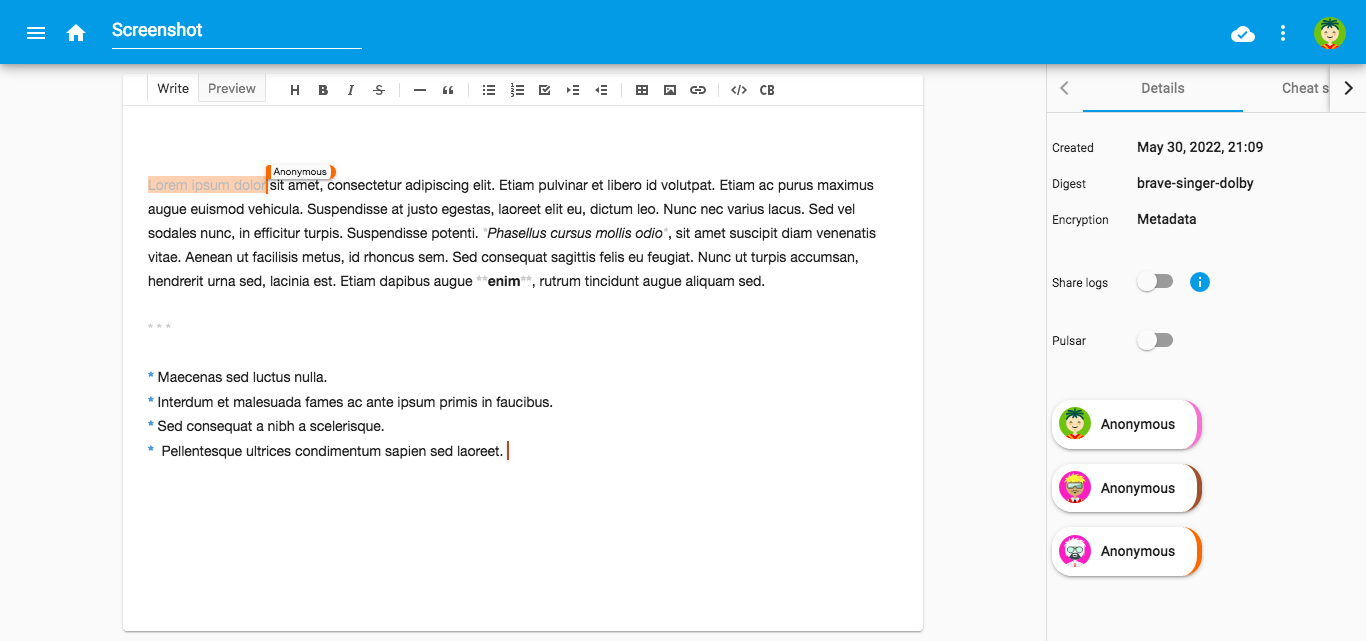
\includegraphics[width=\linewidth]{img/screenshot-mute-editor.png}
    \caption{Capture d'écran d'une session d'édition collaborative avec MUTE}
    \label{fig:interface-mute-editor}
\end{figure}

Pour garantir la confidentialité des échanges, \ac{MUTE} utilise un protocole de génération de clés de groupe.
Ce protocole permet d'établir une clé de chiffrement connue seulement des pairs actuellement connectés, qui est ensuite utilisée pour chiffrer les messages entre pairs.
Ce protocole permet de garantir les propriétés de \emph{backward secrecy} et de \emph{forward secrecy}.
\begin{definition}[Backward Secrecy]
    \label{def:backward-secrecy}
    La \emph{Backward Secrecy} est une propriété de sécurité garantissant qu'un nouveau noeud ne pourra pas déchiffrer avec la nouvelle clé de chiffrement les anciens messages chiffrés avec une clé de chiffrement précédente.
\end{definition}
\begin{definition}[Forward Secrecy]
    \label{def:forward-secrecy}
    La \emph{Forward Secrecy} est une propriété de sécurité garantissant qu'un nouveau noeud ne pourra pas déchiffrer avec la nouvelle clé de chiffrement les futurs messages chiffrés avec une prochaine clé de chiffrement.
\end{definition}

Une copie locale du document est sauvegardée dans le navigateur, avec l'ensemble des modifications.
L'utilisateur-rice peut ainsi accéder à ses documents même sans connexion internet, pour les consulter ou modifier.
Les modifications effectuées dans ce mode hors-ligne seront partagées aux collaborateur-rices à la prochaine connexion de l'utilisateur-rice.

Finalement, la page d'accueil de l'application permet aussi de lister ses documents.
L'utilisateur-rice peut ainsi facilement parcourir ses documents, récupérer leur url pour les partager ou encore supprimer leur copie locale.
\autoref{fig:interface-mute-document-list} illustre cette page de l'application.
\begin{figure}[!ht]
    \centering
    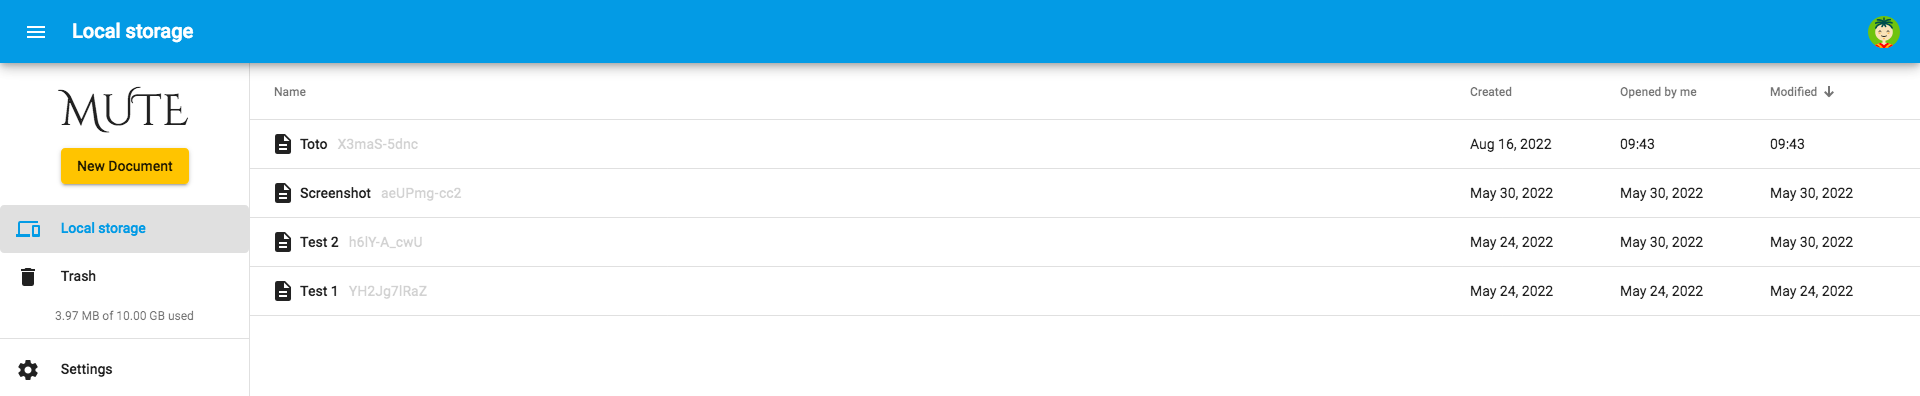
\includegraphics[width=\linewidth]{img/screenshot-mute-document-list.png}
    \caption{Capture d'écran de la liste des documents.}
    \label{fig:interface-mute-document-list}
\end{figure}


\subsection{Architecture système}
Nous représentons l'architecture système d'une collaboration utilisant MUTE par la \autoref{fig:architecture-sys-mute}.

\begin{figure}[!ht]
  \centering
  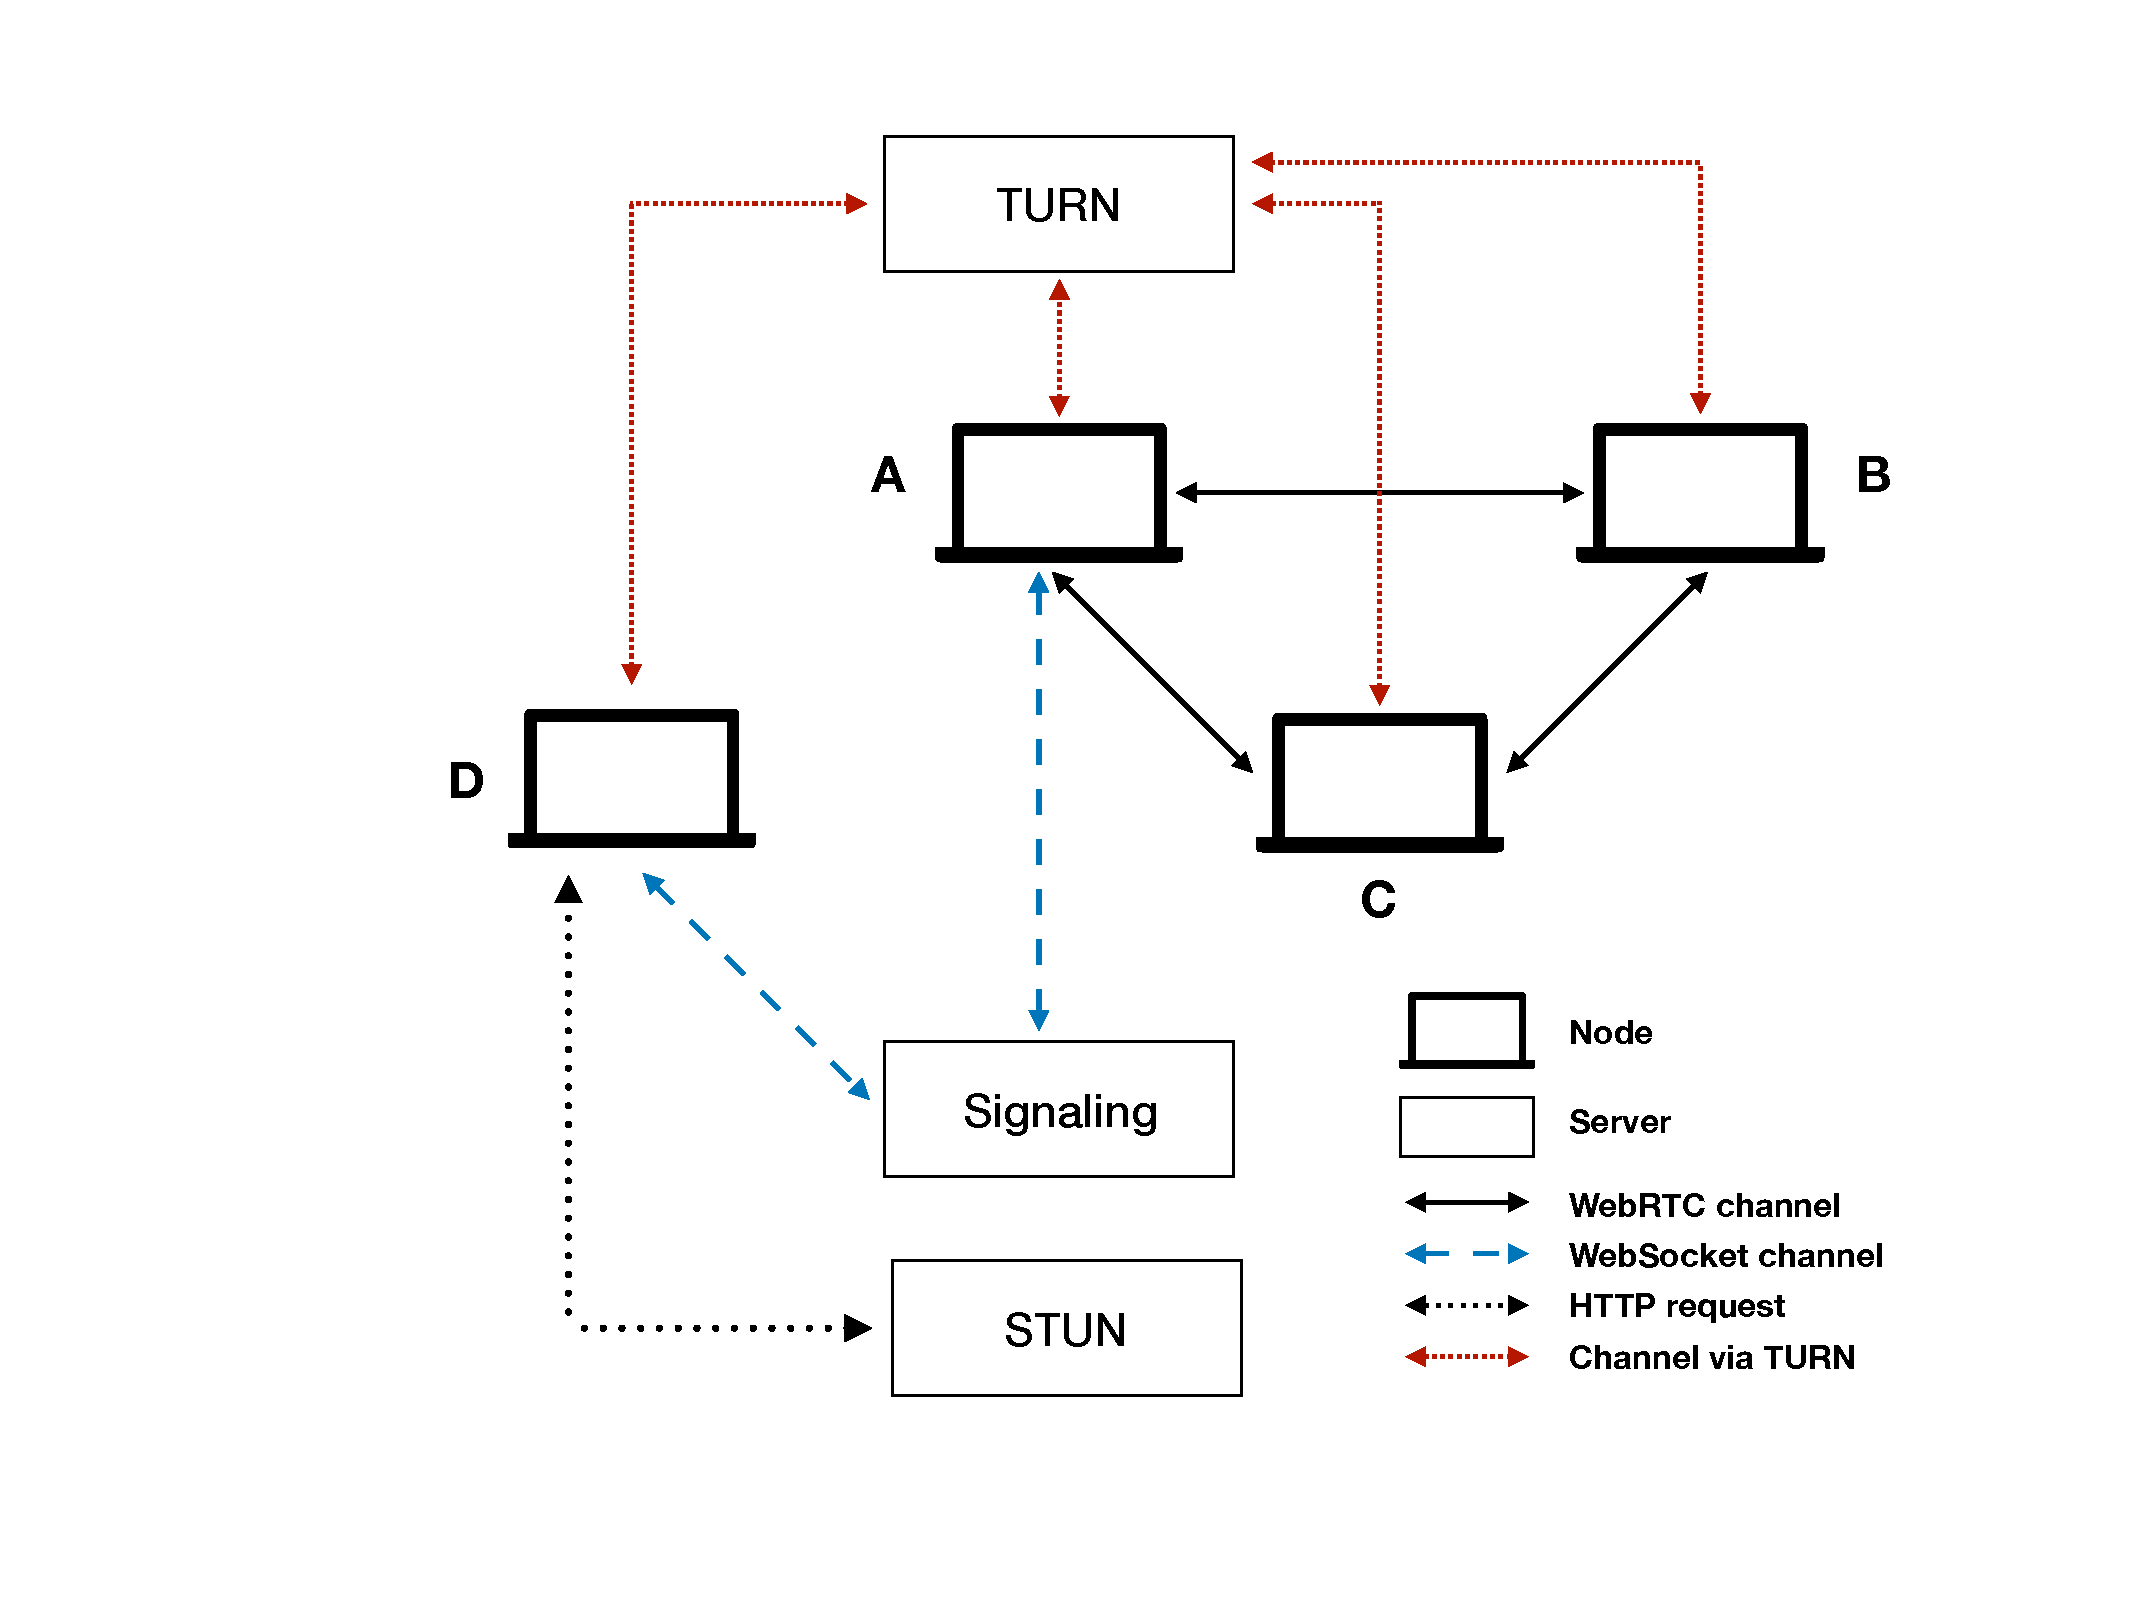
\includegraphics[page=1, trim=0cm 0cm 0cm 0cm, clip, width=.7\linewidth]{img/mute-figures.pdf}
  \caption{Architecture système de l'application MUTE}
  \label{fig:architecture-sys-mute}
\end{figure}

Plusieurs types de noeuds composent cette architecture.
Nous décrivons ci-dessous le type de chacun de ces noeuds ainsi que leurs rôles.

\subsubsection{Pairs}

Au centre de la collaboration se trouvent les noeuds qui correspondent aux utilisateur-rices de l'application et à leurs appareils.
Chaque noeud correspond à une instance de l'application \ac{MUTE}, \ie l'éditeur collaboratif de texte.
Chacun de ces noeuds peut donc consulter des documents et les modifier.

Ces noeuds forment un réseau \ac{P2P}, qui leur permet d'échanger directement notamment pour diffuser les modifications effectuées sur le document.
Les pairs interagissent aussi avec les autres types de noeuds, que nous décrivons dans les parties suivantes.

Notons qu'un noeud peut toutefois être déconnecté du système, \ie dans l'incapacité de se connecter aux autres pairs et d'interagir avec les autres types de noeuds.
Cela ne l'empêche toutefois pas l'utilisateur-rice d'utiliser \ac{MUTE}.

\subsubsection{Services réseaux}

Nous décrivons par cette appelation l'ensemble des composants nécessaires à l'établissement et le bon fonctionnement du réseau \ac{P2P} entre les appareils des utilisateur-rices.

Il s'agit de serveurs ayant pour buts de :
\begin{enumerate}
    \item Permettre à un pair d'obtenir les informations sur son propre état nécessaires pour l'établissement de connexions \ac{P2P}.
    \item Permettre à un pair de découvrir les autres pairs travaillant sur le même document et d'établir une connexion avec eux.
    \item Permettre à des pairs de communiquer même si leur configurations réseaux respectives empêchent l'établissement d'une connection \ac{P2P} directe.
\end{enumerate}

Nous détaillons plus précisément chacun de ces services et les interactions entre les pairs et ces derniers dans la \autoref{sec:mute-couche-reseau}.

\subsubsection{Services sécurité}

Nous décrivons par cette appelation l'ensemble des composants nécessaires à l'authentification des utilisateur-rices et à l'établissement de clés de groupe de chiffrement.

Il s'agit de serveurs ayant pour buts de :
\begin{enumerate}
    \item Permettre à un pair de s'authentifier.
    \item Permettre à un pair de faire connaître sa clé publique de chiffrement.
    \item Vérifier l'identité d'un pair.
    \item Permetttre à un pair de vérifier le comportement honnête du ou des serveurs servant les clés publiques de chiffrement.
\end{enumerate}

Nous dédions la \autoref{sec:mute-couche-securite} à la description de ces différents services et les interactions des pairs avec ces derniers.


\subsection{Architecture logicielle}
Nous décrivons l'architecture logicielle d'un pair, \ie d'une instance de l'application \ac{MUTE} dans un navigateur, dans la \autoref{fig:architecture-log-mute}.

\begin{figure}[!ht]
  \centering
  \includegraphics[page=2, trim=0cm 0cm 0cm 0cm, clip, width=.7\linewidth]{img/mute-figures.pdf}
  \caption{Architecture logicielle de l'application MUTE}
  \label{fig:architecture-log-mute}
\end{figure}

Cette architecture logicielle se compose de plusieurs composants, que nous regroupons par couche.
Chacune de ces couches possède un rôle, que nous présentons brièvement ci-dessous avant de les décrire de manière plus détaillée dans leur section respective.
\begin{enumerate}
    \item La couche \emph{interface utilisateur}, qui regroupe l'ensemble des composants permettant de communiquer des informations aux pairs et avec lesquelles ils peuvent interagir, \ie le document lui-même, son titre mais aussi la liste des collaborateur-rices actuellement connectés.
        Cette couche se charge de transmettre les actions de l'utilisateur-rice aux couches inférieures, et inversement de présenter à l'utilisateur-rice les modifications effectuées par ses pairs.
    \item La couche \emph{réplication}, qui regroupe l'ensemble des composants permettant de représenter les données répliquées entre pairs, \ie les \acp{CRDT} utilisés pour représenter le document, ses métadonnées (titre, date de création...), l'ensemble des collaborateurs et leur curseur.
        Cette couche se charge d'intégrer les modifications effectuées par l'utilisateur-rice et de transmettre les opérations correspondantes aux couches inférieures, et inversement d'intégrer les opérations effectuées par ses pairs et d'indiquer à la couche \emph{interface utilisateur} les modifications correspondantes.
    \item La couche \emph{livraison}, qui est constitué d'un unique composant permettant de garantir les modèles de livraison requis par les différents \acp{CRDT} implémentés pour représenter le document.
        Cette couche se charge d'adjoindre aux opérations de l'utilisateur-rice leur(s) dépendance(s) avant de les transmettre aux couches inférieures, et de livrer les opérations de ses pairs une fois leur(s) dépendance(s) livrées au préalable, ou de les mettre en attente le cas échéant.
    \item La couche \emph{sécurité}, qui est constitué d'un unique composant gérant le chiffrement des messages.
        Cette couche se charge d'établir la clé de chiffrement de groupe, puis de chiffrer les messages de l'utilisateur-rice avec cette dernière avant de les transmettre à la couche inférieure, et inversement de déchiffrer les messages chiffrés de ses pairs avant de les transmettre aux couches supérieures.
    \item La couche \emph{réseau}, qui est constitué d'un unique composant permettant d'interagir avec le réseau \ac{P2P}.
        Cette couche se charge d'établir les connexions \ac{P2P}, puis permet de diffuser les messages chiffrés de l'utilisateur-rice à un ou plusieurs de ses pairs, et inversement de transmettre les messages chiffrés de ses pairs à la couche supérieure.
\end{enumerate}



\section{Couche interface utilisateur}
Comme illustré par la \autoref{fig:interface-mute-editor}, l'interface de la page d'un document se compose principalement d'un éditeur de texte.
Ce dernier supporte le langage de balisage Markdown \cite{2004-markdown}.
Ainsi, l'éditeur permet d'inclure plusieurs éléments légers de style.
Les balises du langage Markdown étant du texte, elles sont répliquées nativement par le \ac{CRDT} utilisé en interne par \ac{MUTE} pour représenter la séquence.\\

L'interface de la page de l'éditeur de document est agrémentée de plusieurs mécanismes permettant d'établir une conscience de groupe entre les collaborateur-rices.
L'indicateur en haut à droite de la page représente le statut de connexion de l'utilisateur-rice.
Celui-ci permet d'indiquer à l'utilisateur-rice s'iel est actuellement connecté-e au réseau \ac{P2P}, en cours de connexion, ou si un incident réseau a lieu.

De plus, \ac{MUTE} affiche sur la droite de l'éditeur la liste des collaborateur-rices actuellement connecté-es.
Un curseur ou une sélection distante est associée pour chaque membre de la liste.
Ces informations permettent d'indiquer à l'utilisateur-rice dans quelles sections du document ses collaborateur-rices sont en train de travailler.
Ainsi, iels peuvent se répartir la rédaction du document de manière implicite ou suivre facilement les modifications d'un-e collaborateur-rice.\\

Bien que fonctionnelle, cette interface souffre néanmoins de plusieurs limites.
Notamment, nous n'avons pas encore pu étudier la littérature concernant les mécanismes de conscience pour supporter la collaboration, au-delà du système de curseurs distants.

Nous identifions ainsi plusieurs axes de travail pour ces mécanismes.
Tout d'abord, l'axe des \emph{mécanismes de conscience des changements}.
Le but serait de proposer des mécanismes pour :
\begin{enumerate}
    \item Mettre en lumière de manière intelligible les modifications effectuées par les collabateur-rices dans le cadre de collaborations temps réel à large échelle.
        Un tel mécanisme représente un défi de part le débit important de changements, potentiellement à plusieurs endroits du document de manière quasi-simultanée, à présenter à l'utilisateur-rice.
    \item Mettre en lumière de manière intelligible les modifications effectuées par les collaborateur-rices dans le cadre de collaborations asynchrones.
        De nouveau, ce mécanisme représente un défi de part la quantité massive de changements, une fois encore potentiellement à plusieurs endroits du document, à présenter à l'utilisateur-rice.
\end{enumerate}
Une piste de travail potentiellement liée serait l'ajout d'une fonctionnalité d'historique du document, permettant aux utilisateur-rices de parcourir ses différentes versions obtenues au fur et à mesure des modifications.
L'intégration d'une telle fonctionnalité dans un éditeur \ac{P2P} pose cependant plusieurs questions : quel historique présenter aux utilisateur-rices, sachant que chacun-e a potentiellement observé un ordre différent des modifications ?
Doit-on convenir d'une seule version de l'historique ?
Dans ce cas, comment choisir et construire cet historique ?\\

Le second axe de travail sur les mécanismes de conscience concerne les \emph{mécanismes de conscience de groupe}.
Actuellement, nous affichons l'ensemble des collaborateur-rices actuellement connecté-es.
Cette approche s'avère lourde voire entravante dans le cadre de collaborations à large échelle où le nombre de collaborateur-rices dépasse plusieurs centaines.
Il convient donc de déterminer quelles informations présenter à l'utilisateur-rice dans cette situation, \eg une liste compacte de pairs et leur curseur respectif, ainsi que le nombre de pairs total.\\

Ainsi, pour chacun de ses axes d'amélioration, il convient d'étudier leur littérature respective et de déterminer les solutions proposées qui sont adaptées à \ac{MUTE}.


\section{Couche réplication}

\subsection{Modèle de données du document texte}
\label{sec:mute-crdts}

MUTE propose plusieurs alternatives pour représenter le document texte.
MUTE permet de soit utiliser une implémentation de LogootSplit\footnote{Les deux implémentations proviennent de la librairie \texttt{mute-structs} : \url{https://github.com/coast-team/mute-structs}}, soit de RenamableLogootSplit\footnotemark[\value{footnote}] ou soit de Dotted LogootSplit \footnote{Implémentation fournie par la librairie suivante : \url{https://github.com/coast-team/dotted-logootsplit}}.
Ce choix est effectué via une valeur de configuration de l'application choisie au moment de son déploiement.

Le modèle de données utilisé interagit avec l'éditeur de texte par l'intermédiaire d'opérations textes.
Lorsque l'utilisateur effectue des modifications locales, celles-ci sont détectées et mises sous la forme d'opérations textes.
Elles sont transmises au modèle de données, qui les intègre alors à la structure de données répliquées.
Le \ac{CRDT} retourne en résultat l'opération distante à propager aux autres noeuds.

De manière complémentaire, lorsqu'une opération distante est livrée au modèle de données, elle est intégrée par le \ac{CRDT} pour actualiser son état.
Le \ac{CRDT} génère les opérations textes correspondantes et les transmet à l'éditeur de texte pour mettre à jour la vue.

En plus du texte, MUTE maintient un ensemble de métadonnées par document.
Par exemple, les utilisateurs peuvent donner un titre au document.
Pour représenter cette donnée additionnelle, nous associons un Last-Writer-Wins Register \ac{CRDT} synchronisé par opérations \cite{shapiro_2011_crdt} au document.
De façon similaire, nous utilisons un First-Writer-Wins Register \ac{CRDT} synchronisé par opérations pour représenter la date de création du document.


\subsection{Module de livraison des opérations}
\label{sec:mute-delivery-model}

Comme indiqué précédemment, la couche livraison est formée d'un unique composant, que nous nommons module de livraison.
Ce module est associé aux \acp{CRDT} synchronisés par opérations représentant le document texte, \ie LogootSplit ou RenamableLogootSplit.

Le rôle de ce module est de garantir que le modèle de livraison des opérations requis par le \ac{CRDT} pour assurer la convergence à terme \cf{def:eventual-consistency} soit satisfait, \ie que l'ensemble des opérations soient livrées dans un ordre correct à l'ensemble des noeuds.

Pour cela, le module de livraison doit implémenter les contraintes imposées par ces \acp{CRDT} sur l'ordre de livraison des opérations (cf. \autoref{def:ls-delivery-model}, page \pageref{def:ls-delivery-model} et \autoref{def:rls-delivery-model}, page \pageref{def:ls-delivery-model}).
Pour rappel, le modèle de livraison de RenamableLogootSplit est le suivant :
\begin{enumerate}
    \item Une opération doit être livrée à l'ensemble des noeuds à terme.
    \item Une opération doit être livrée qu'une seule et unique fois aux noeuds.
    \item Une opération \emph{remove} doit être livrée à un noeud une fois que les opérations \emph{insert} des éléments concernés par la suppression ont été livrées à ce dernier.
    \item Une opération peut être délivrée à un noeud qu'à partir du moment où l'opération \emph{rename} qui a introduit son époque de génération a été délivrée à ce même noeud.
\end{enumerate}

Nous décrivons ci-dessous comment nous assurons chacune de ces contraintes.


\subsubsection{Livraison des opérations en exactement un exemplaire}
\label{sec:mute-exactly-once-delivery}

Afin de respecter la contrainte de livraison en exactement un exemplaire, il est nécessaire d'identifier de manière unique chaque opération.
Pour cela, le module de livraison ajoute un \emph{Dot} \cite{2014-scalable-accurate-causality-tracking} à chaque opération :

\begin{definition}[Dot]
  \label{def:dot}
  Un \emph{Dot} est une paire $\langle \trm{nodeId}, \trm{nodeSyncSeq}\rangle$ où
  \begin{enumerate}
    \item $\trm{nodeId}$, l'identifiant unique du noeud qui a généré l'opération.
    \item $\trm{nodeSyncSeq}$, le numéro de séquence courant du noeud à la génération de l'opération.
  \end{enumerate}
\end{definition}

Il est à noter que \emph{nodeSyncSeq} est différent du \emph{nodeSeq} utilisé dans LogootSplit et RenamableLogootSplit \cf{sec:logootsplit}.
En effet, \emph{nodeSyncSeq} se doit d'augmenter à chaque opération tandis que \emph{nodeSeq} n'augmente qu'à la création d'un nouveau bloc, \ie lors d'une insertion ou d'un renommage.
Les contraintes étant différentes, il est nécessaire de distinguer ces deux données.\\

Chaque noeud maintient une structure de données représentant l'ensemble des opérations reçues par le pair.
Elle permet de vérifier à la réception d'une opération si le dot de cette dernière est déjà connu.
S'il s'agit d'un nouveau dot, le module de livraison peut livrer l'opération au \ac{CRDT} et ajouter son dot à la structure.
Le cas échéant, cela indique que l'opération a déjà été livrée précédemment et doit être ignorée cette fois-ci.

Plusieurs structures de données sont adaptées pour maintenir l'ensemble des opérations reçues.
Dans le cadre de MUTE, nous avons choisi d'utiliser un vecteur de version.
Cette structure nous permet de réduire à un dot par noeud le surcoût en métadonnées du module de livraison, puisqu'il ne nécessite que de stocker le dot le plus récent par noeud.
Cette structure permet aussi de vérifier en temps constant si une opération est déjà connue.
La \autoref{fig:exactly-once-delivery} illustre son fonctionnement.\\

\begin{figure}[!ht]
  \subfloat[Exécution avec livraison multiple d'une opération $\trm{insert}$]{
      \begin{minipage}{\linewidth}
          \centering
          \resizebox{\columnwidth}{!}{
            \begin{tikzpicture}
                \path
                    node {\textbf{A}}
                    ++(0:0.5 * \widthletter) node[epoch] {\epoch{0}}
                    ++(0:1.05 * \widthoriginepoch) node[block, label=below:{\id{p}{A0}{0..4}}] (S0A) {OGNON}
                    ++(0:5 * \widthletter) node[epoch] (S1A-left) {\epoch{0}}
                    ++(0:1.05* \widthoriginepoch) node[letter, label=below:{\id{p}{A0}{0}}]  {O}
                    ++(0:\widthletter) node[letter, fill=mydarkorange, label=above:{\id{p}{A0}{0}\id{m}{A1}{0}}] {I}
                    ++(0:\widthletter) node[block, label=below:{\id{p}{A0}{1..4}}] (S1A-right) {GNON}
                    ++(0:21 * \widthletter) node[epoch] (S2A-left) {\epoch{0}}
                    ++(0:1.05 * \widthoriginepoch) node[letter, label=below:{\id{p}{A0}{0}}] {O}
                    ++(0:\widthletter) node[block, label=below:{\id{p}{A0}{1..4}}] {GNON};


                \path
                    ++(270:4) node {\textbf{B}}
                    ++(0:0.5 * \widthletter) node[epoch] {\epoch{0}}
                    ++(0:1.05 * \widthoriginepoch) node[block, label=below:{\id{p}{A0}{0..4}}] (S0B) {OGNON}
                    ++(0:12 * \widthletter) node[epoch] (S1B-left) {\epoch{0}}
                    ++(0:1.05 * \widthoriginepoch) node[letter, label=below:{\id{p}{A0}{0}}] {O}
                    ++(0:\widthletter) node[letter, fill=mydarkorange, label=above:{\id{p}{A0}{0}\id{m}{A1}{0}}] {I}
                    ++(0:\widthletter) node[block, label=below:{\id{p}{A0}{1..4}}] (S1B-right) {GNON}
                    ++(0:5 * \widthletter) node[epoch] (S2B-left) {\epoch{0}}
                    ++(0:1.05 * \widthoriginepoch) node[letter, label=below:{\id{p}{A0}{0}}] {O}
                    ++(0:\widthletter) node[block, label=below:{\id{p}{A0}{1..4}}] (S2B-right) {GNON}
                    ++(0:8 * \widthletter) node[epoch] (S3B-left) {\epoch{0}}
                    ++(0:1.05 * \widthoriginepoch) node[letter, label=below:{\id{p}{A0}{0}}] {O}
                    ++(0:\widthletter) node[block, label=below:{\id{p}{A0}{1..4}}] {GNON};

                \draw[->, thick]
                  (S0A) edge node[above, align=center]{\emph{insert "I"}\\\emph{between}\\\emph{"O" and "G"}} (S1A-left)
                  (S1B-right) edge node[above, align=center]{\emph{remove "I"}} (S2B-left);

                \draw[dotted]
                  (S1A-right) -- (S2A-left)
                  (S0B) -- (S1B-left)
                  (S2B-right) -- (S3B-left);

                \draw[dashed, ->, thick, shorten >= 3]
                  (S1A-right.east) edge node[right, align=center]{\emph{insert "I" at} {\color{mydarkorange}\id{p}{A0}{0}\id{m}{A1}{0}}}  (S1B-left.west)
                  (S1A-right.east) edge node[right, align=center]{\emph{insert "I" at} {\color{mydarkorange}\id{p}{A0}{0}\id{m}{A1}{0}}}  (S3B-left.west)
                  (S2B-right.east) edge node[below right, align=center]{$\trm{rmv}$ {\color{mydarkorange}\id{i}{B0}{1..1}}} (S2A-left.west);
            \end{tikzpicture}
            \label{fig:exactly-once-delivery-rls}
          }
          \end{minipage}
        }
        \hfil
  \subfloat[État et comportement du module de livraison au cours de l'exécution décrite en \autoref{fig:exactly-once-delivery-rls}]{
    \begin{minipage}{\linewidth}
      \centering
      \resizebox{\columnwidth}{!}{
        \begin{tikzpicture}
            \path
                node {\textbf{A}}
                ++(0:1) node[point, label=above:{$\langle A:5 \rangle$}] (a-start) {}
                ++(0:2) node[draw, circle, label=above:{$\langle A:6 \rangle$}] (a-a6) {a6}
                ++(0:8) node[point, label=above:{$\langle A:6,B:1 \rangle$}, label=below:{\emph{deliver}}] (a-b1) {}
                ++(0:3) node (a-end) {};


            \path
                ++(270:3) node {\textbf{B}}
                ++(0:1) node[point, label=below:{$\langle A:5 \rangle$}] (b-start) {}
                ++(0:5) node[point, label=below:{$\langle A:6 \rangle$}, label=above:{\emph{deliver}}] (b-a6-1) {}
                ++(0:2) node[draw, circle, label=below:{$\langle A:6,B:1 \rangle$}] (b-b1) {b1}
                ++(0:5) node[point, label=below:{$\langle A:6,B:1 \rangle$}, label=above:{\emph{discard}}] (b-a6-2) {}
                ++(0:1) node (b-end) {};

            \draw[->, thick]
              (a-start) edge (a-a6)
              (b-a6-1) edge (b-b1);

            \draw[dotted]
              (a-a6) -- (a-b1) -- (a-end)
              (b-start) -- (b-a6-1)
              (b-b1) -- (b-end);

            \draw[dashed, ->, thick, shorten >= 3]
              (a-a6.east) edge (b-a6-1.west)
              (a-a6.east) edge (b-a6-2.west)
              (b-b1.east) edge (a-b1.west);
        \end{tikzpicture}
        \label{fig:exactly-once-delivery-sync}
      }
      \end{minipage}
    }
  \caption{Gestion de la livraison en exactement un exemplaire des opérations}
  \label{fig:exactly-once-delivery}
\end{figure}

Dans cet exemple, qui reprend celui de la \autoref{fig:why-exactly-once-delivery}, deux noeuds A et B répliquent une séquence.
Initialement, celle-ci contient les éléments "OGNON".
Ces éléments ont été insérés un par un par le noeud A, donc par le biais des opérations \emph{a1} à \emph{a5}.
Le module de livraison de chaque noeud maintient donc initialement le vecteur de version $\langle A:5 \rangle$.

Le noeud A insère l'élément "I" entre les éléments "O" et "G".
Cette modification est alors labellisée \emph{a6} par son module de livraison et est envoyée au noeud B.
À la réception de cette opération, le module de B compare son dot avec son vecteur de version local.
L'opération \emph{a6} étant la prochaine opération attendue de A, celle-ci est acceptée : elle est alors livrée au \ac{CRDT} et le vecteur de version est mis à jour.

Le noeud B supprime ensuite l'élément nouvellement inséré.
S'agissant de la première modification de B, cette modification \emph{b1} ajoute l'entrée correspondante dans le vecteur de version $\langle A:6, B:1 \rangle$.
L'opération est envoyée au noeud A.
Cette opération étant la prochaine opération attendue de B, elle est acceptée et livrée.

Finalement, le noeud B reçoit de nouveau l'opération \emph{a6}.
Son module de livraison détermine alors qu'il s'agit d'un doublon : l'opération apparaît déjà dans le vecteur de version $\langle A:6, B:1 \rangle$.
L'opération est donc ignorée, et la résurgence de l'élément "I" illustrée dans la \autoref{fig:why-exactly-once-delivery} est évitée.\\

Il est à noter que dans le cas où un noeud reçoit une opération avec un dot plus élevé que celui attendu (\eg le noeud A reçoit une opération \emph{b3} à la fin de l'exemple), cette opération est mise en attente.
En effet, livrer cette opération nécessiterait de mettre à jour le vecteur de version à $\langle A:6,B:3 \rangle$ et masquerait le fait que l'opération \emph{b2} n'a jamais été reçue.
L'opération \emph{b3} est donc mise en attente jusqu'à la livraison de l'opération \emph{b2}.

Ainsi, l'implémentation de livraison en exactement un exemplaire d'une opération avec un vecteur de version comme structure de données force une livraison \ac{FIFO} des opérations par noeuds.
Il s'agit d'une contrainte non-nécessaire et qui peut introduire des délais dans la collaboration, notamment si une opération d'un noeud est perdue par le réseau.
Nous jugeons cependant acceptable ce compromis entre le surcoût du mécanisme de livraison en exactement un exemplaire et son impact sur l'expérience utilisateur.\\

Pour retirer cette contrainte superflue, il est possible de remplacer cette structure de données par un \emph{Interval Version Vector} \cite{2014-optimized-or-sets}.
Au lieu d'enregistrer seulement le dernier dot intégré par noeud, cette structure de données enregistre les intervalles de dots intégrés.
Ceci permet une livraison \emph{dans le désordre} des opérations, \ie une livraison des opérations dans un ordre différent de leur ordre d'émission, tout en garantissant une livraison en exactement un exemplaire et en compactant efficacement les données stockées par le module de livraison à terme.


\subsubsection{Livraison de l'opération \emph{remove} après l'opération \emph{insert}}
La seconde contrainte que le modèle de livraison doit respecter spécifie qu'une opération $\trm{remove}$ doit être livrée après les opérations $\trm{insert}$ insérant les éléments concernés.

Pour cela, le module de livraison ajoute un ensemble \emph{Deps} à chaque opération $\trm{remove}$ avant de la diffuser :

\begin{definition}[Deps]
  \emph{Deps} est un ensemble d'opérations.
  Il représente l'ensemble des opérations dont dépend l'opération $\trm{remove}$ et qui doivent donc être livrées au préalable.
\end{definition}

Plusieurs structures de données sont adaptées pour représenter les dépendances de l'opération $\trm{remove}$.
Dans le cadre de MUTE, nous avons choisi d'utiliser un ensemble de dots : pour chaque élément supprimé par l'opération $\trm{remove}$, nous identifions le noeud l'ayant inséré et nous ajoutons le dot correspondant à l'opération la plus récente de ce noeud à l'ensemble des dépendances.
Cette approche nous permet de limiter à un dot par élément supprimé le surcoût en métadonnées des dépendances et de les calculer en un temps linéaire par rapport au nombre d'éléments supprimés.
Nous illustrons le calcul et l'utilisation des dépendances de l'opération $\trm{remove}$ à l'aide de la \autoref{fig:causal-remove-delivery}.\\

\begin{figure}[!ht]
  \subfloat[Exécution avec livraison dans le désordre d'une insertion et de sa suppression]{
      \begin{minipage}{\linewidth}
          \centering
          \resizebox{\columnwidth}{!}{
            \begin{tikzpicture}
              \newcommand\initialstate[3]{
                \path
                  #1
                  ++#2
                  ++(0:0.5) node[epoch] {\epoch{0}}
                  ++(0:1.05 * \widthoriginepoch) node[block, label=#3:{$\betterid{p}{A1}{0..3}$}] {WOLD};
              }

              \newcommand\insr[3]{
                \path
                  #1
                  ++#2
                  ++(0:0.5) node[epoch] {\epoch{0}}
                  ++(0:1.05 * \widthoriginepoch) node[block, label=#3:{$\betterid{p}{A1}{0..1}$}] {WO}
                  ++(0:\widthblock) node[letter, fill=\colorblockone, label=-#3:{$\coloridone\betterid{p}{A1}{1}\betterid{m}{A2}{0}$}] {R}
                  ++(0:\widthletter)  node[block, label=#3:{$\betterid{p}{A1}{2..3}$}] {LD};
              }

              \newcommand\rmvr[3]{
                \path
                  #1
                  ++#2
                  ++(0:0.5) node[epoch] {\epoch{0}}
                  ++(0:1.05 * \widthoriginepoch) node[block, label=#3:{$\betterid{p}{A1}{0..1}$}] {WO}
                  ++(0:\widthblock)  node[block, label=#3:{$\betterid{p}{A1}{2..3}$}] {LD};
              }

              \newcommand\offseta{ (90:1.2) }
              \newcommand\offsetb{ (270:1.2) }

              \path
                node {\textbf{A}}
                ++(0:0.5) node (a) {}
                +(0:24) node (a-end) {}
                +(0:1) node[point] (a-initial) {}
                +(0:6) node[point, label=-170:{$\trm{ins}(O \prec R \prec K)$}, label={[xshift=6em]-10:{$\trm{ins}(\betterepoch{0},{\coloridone\betterid{p}{A1}{1}\betterid{m}{A2}{0}},R)$}}] (a-ins-r) {}
                +(0:16) node[point] (a-recv-rmv-r) {}
                +(0:19) node (a-last-display) {}
                +(0:23) node (a-final) {};

              \initialstate{(a-initial)}{\offseta}{90};
              \insr{(a-ins-r)}{\offseta}{90};
              \rmvr{(a-last-display)}{\offseta}{90};

              \draw[dotted] (a) -- (a-initial) (a-final) -- (a-end);
              \draw[->, thick] (a-initial) --  (a-ins-r) -- (a-recv-rmv-r) -- (a-final);

              \path
                ++(270:3) node {\textbf{B}}
                ++(0:0.5) node (b) {}
                +(0:24) node (b-end) {}
                +(0:1) node[point] (b-initial) {}
                +(0:8) node[point] (b-recv-ins-r) {}
                +(0:14) node[point, label=170:{$\trm{rmv}(R)$}, label={[xshift=1em]10:{$\trm{rmv}(\betterepoch{0},{\coloridone\betterid{p}{A1}{1}\betterid{m}{A2}{0}})$}}] (b-rmv-r) {}
                +(0:19) node (b-last-display) {}
                +(0:23) node (b-final) {};

              \initialstate{(b-initial)}{\offsetb}{-90};
              \insr{(b-recv-ins-r)}{\offsetb}{-90};
              \rmvr{(b-last-display)}{\offsetb}{-90};

              \draw[dotted] (b) -- (b-initial) (b-final) -- (b-end);
              \draw[->, thick] (b-initial) --  (b-recv-ins-r) -- (b-rmv-r) -- (b-final);

              \path
                ++(270:6) node {\textbf{C}}
                ++(0:0.5) node (c) {}
                +(0:24) node (c-end) {}
                +(0:1) node[point] (c-initial) {}
                +(0:16) node[point] (c-recv-rmv-r) {}
                +(0:19) node[point] (c-recv-ins-r) {}
                +(0:23) node (c-final) {};

              \initialstate{(c-initial)}{\offsetb}{-90};
              \initialstate{(c-recv-rmv-r)}{\offsetb}{-90};
              \initialstate{(c-recv-ins-r)}{\offsetb}{-90};

              \draw[dotted] (c) -- (c-initial) (c-final) -- (c-end);
              \draw[->, thick] (c-initial) --  (c-recv-rmv-r) -- (c-recv-ins-r) -- (c-final);

              \draw[->, dashed, shorten >= 1] (a-ins-r) -- (b-recv-ins-r);
              \draw[->, dashed, shorten >= 1] (a-ins-r) -- (c-recv-ins-r);
              \draw[->, dashed, shorten >= 1] (b-rmv-r) -- (a-recv-rmv-r);
              \draw[->, dashed, shorten >= 1] (b-rmv-r) -- (c-recv-rmv-r);
            \end{tikzpicture}
            \label{fig:causal-remove-delivery-rls}
          }
          \end{minipage}
        }
        \hfil
  \subfloat[État et comportement du module de livraison au cours de l'exécution décrite en \autoref{fig:causal-remove-delivery-rls}]{
    \begin{minipage}{\linewidth}
      \centering
      \resizebox{\columnwidth}{!}{
        \begin{tikzpicture}
          \path
            node {\textbf{A}}
            ++(0:0.5) node (a) {}
            +(0:24) node (a-end) {}
            +(0:1) node[point, label=above right:{$\langle A:4 \rangle$}] (a-initial) {}
            +(0:6) node[point, label=-170:{\emph{tag as} $a_5$}, label=10:{$\langle A:5 \rangle$}] (a-ins-r) {}
            +(0:16) node[point,label={[xshift=-10pt]-170:{\emph{deliver} $b_1$}}, label=10:{$\langle A:5,B:1 \rangle$}] (a-recv-rmv-r) {}
            +(0:19) node (a-last-display) {}
            +(0:23) node (a-final) {};

          \draw[dotted] (a) -- (a-initial) (a-final) -- (a-end);
          \draw[->, thick] (a-initial) --  (a-ins-r) -- (a-recv-rmv-r) -- (a-final);

          \path
            ++(270:3) node {\textbf{B}}
            ++(0:0.5) node (b) {}
            +(0:24) node (b-end) {}
            +(0:1) node[point, label=-10:{$\langle A:4 \rangle$}] (b-initial) {}
            +(0:8) node[point, label={[xshift=-10pt]170:{\emph{deliver} $a_5$}}, label=-10:{$\langle A:5 \rangle$}] (b-recv-ins-r) {}
            +(0:14) node[point, label=170:{\emph{tag as} $b_1$}, label={[xshift=10pt]-10:{$\langle A:5,B:1 \rangle$}}] (b-rmv-r) {}
            +(0:19) node (b-last-display) {}
            +(0:23) node (b-final) {};

          \draw[dotted] (b) -- (b-initial) (b-final) -- (b-end);
          \draw[->, thick] (b-initial) --  (b-recv-ins-r) -- (b-rmv-r) -- (b-final);

          \path
            ++(270:6) node {\textbf{C}}
            ++(0:0.5) node (c) {}
            +(0:24) node (c-end) {}
            +(0:1) node[point, label=-10:{$\langle A:4 \rangle$}] (c-initial) {}
            +(0:16) node[point, label={[xshift=-10pt]170:{\emph{postpone} $b_1$}}, label=-90:{$\langle A:4 \rangle$}] (c-recv-rmv-r) {}
            +(0:19) node[point,label={[xshift=0pt,yshift=10pt]90:{\emph{deliver} $a_5$}}, label=-10:{$\langle A:5 \rangle$}] (c-recv-ins-r) {}
            +(0:22) node[point,label={[xshift=0pt]90:{\emph{deliver} $b_1$}}, label=-10:{$\langle A:5,B:1 \rangle$}] (c-recv-rmv-r-2) {}
            +(0:23) node (c-final) {};

          \draw[dotted] (c) -- (c-initial) (c-final) -- (c-end);
          \draw[->, thick] (c-initial) --  (c-recv-rmv-r) -- (c-recv-ins-r) -- (c-recv-rmv-r-2) -- (c-final);

          \draw[->, dashed, shorten >= 1] (a-ins-r) -- (b-recv-ins-r);
          \draw[->, dashed, shorten >= 1] (a-ins-r) -- (c-recv-ins-r);
          \draw[->, dashed, shorten >= 1] (b-rmv-r) edge node[right] {$\{\trm{deps}: \langle A:5 \rangle\}$}  (a-recv-rmv-r);
          \draw[->, dashed, shorten >= 1] (b-rmv-r) edge node[left] {$\{\trm{deps}: \langle A:5 \rangle\}$} (c-recv-rmv-r);

          \draw[->, dotted, thick, shorten >= 1] (c-recv-rmv-r) edge[bend right] (c-recv-rmv-r-2);
        \end{tikzpicture}
        \label{fig:causal-remove-sync}
      }
      \end{minipage}
    }
  \caption{Gestion de la livraison des opérations $\trm{remove}$ après les opérations $\trm{insert}$ correspondantes}
  \label{fig:causal-remove-delivery}
\end{figure}

Dans cet exemple, trois noeuds A, B et C répliquent et éditent collaborativement une séquence.
Les trois noeuds partagent le même état initial : une séquence contenant les éléments "WOLD" et un vecteur de versions $\langle A:4 \rangle$.

Le noeud A insère l'élément "L" entre les éléments "R" et "D".
Cet élément se voit attribué l'identifiant \id{p}{A1}{1}\id{m}{A2}{0}.
L'opération correspondante $a_5$ est diffusée aux autres noeuds.

À la réception de cette dernière, le noeud B supprime l'élément "L" nouvellement inséré et génère l'opération $b_1$ correspondante.
Comme indiqué précédemment, l'opération $b_1$ étant une opération $\trm{remove}$, le module de livraison calcule ses dépendances avant de la diffuser.
Pour chaque élément supprimé ("L"), le module de livraison récupère l'identifiant de l'élément (\id{p}{A1}{1}\id{m}{A2}{0}) et en extrait l'identifiant du noeud qui l'a inséré (A).
Le module ajoute alors le dot de l'opération la plus récente reçue de ce noeud ($\langle A:5 \rangle$) à l'ensemble des dépendances de l'opération.
L'opération est ensuite diffusée.

À la réception de l'opération $b_1$, le noeud A vérifie s'il possède l'ensemble des dépendances de l'opération.
Le noeud A ayant déjà intégré l'opération $a_5$, le module de livraison livre l'opération $b_1$ au \ac{CRDT}.

À l'inverse, lorsque le noeud C reçoit l'opération $b_1$, il n'a pas encore reçu l'opération $a_5$.
L'opération $b_1$ est alors mise en attente.
À la réception de l'opération $a_5$, celle-ci est livrée.
Le module de livraison ré-évalue alors le cas de l'opération $b_1$ et détermine qu'elle peut à présent être livrée.\\

Il est à noter que notre approche pour générer l'ensemble des dépendances est une approximation.
En effet, nous ajoutons les dots des opérations les plus récentes des auteurs des éléments supprimés.
Nous n'ajoutons pas les dots des opérations qui ont spécifiquement inséré les éléments supprimés.
Pour cela, il serait nécessaire de parcourir le journal des opérations à la recherche des opérations $\trm{insert}$ correspondantes.
Cette méthode serait plus coûteuse, sa complexité dépendant du nombre d'opérations dans le journal des opérations, et incompatible avec un mécanisme tronquant le journal des opérations en utilisant la stabilité causale.
Notre approche introduit un potentiel délai dans la livraison d'une opération $\trm{remove}$ par rapport à une livraison utilisant ses dépendances exactes, puisqu'elle va reposer sur des opérations plus récentes et potentiellement encore inconnues par le noeud.
Mais il s'agit là aussi d'un compromis que nous jugeons acceptable entre le surcoût du mécanisme de livraison et l'expérience utilisateur.


\subsubsection{Livraison des opérations après l'opération \emph{rename} introduisant leur époque}
La troisième contrainte spécifiée par le modèle de livraison est qu'une opération doit être livrée après l'opération \emph{rename} qui a introduit son époque de génération.

Pour cela, le module de livraison doit donc récupérer l'époque courante de la séquence répliquée, récupérer le dot de l'opération \emph{rename} l'ayant introduite et l'ajouter en tant que dépendance de chaque opération.
Cependant, dans notre implémentation, le module de livraison et le module représentant la séquence répliquée sont découplés et ne peuvent interagir directement l'un avec l'autre.\\

Pour remédier à ce problème, le module de livraison maintient une structure supplémentaire : un vecteur des dots des opérations \emph{rename} connues.
À la réception d'une opération \emph{rename} distante, l'entrée correspondante de son auteur est mise à jour avec le dot de la nouvelle époque introduite.
À la génération d'une opération locale, l'opération est examinée pour récupérer son époque de génération.
Le module conserve alors seulement l'entrée correspondante dans le vecteur des dots des opérations \emph{rename}.
À ce stade, le contenu du vecteur est ajouté en tant que dépendance de l'opération.
Ensuite, si l'opération locale s'avère être une opération \emph{rename}, le vecteur est modifié pour ne conserver que le dot de l'époque introduite par l'opération.
La \autoref{fig:epoch-based-delivery} illustre ce fonctionnement.\\

\begin{figure}[!ht]
  \subfloat[Exécution]{
      \begin{minipage}{\linewidth}
          \centering
          \resizebox{\columnwidth}{!}{
            \begin{tikzpicture}
              \path
                node {\textbf{A}}
                +(0:20) node (a-end) {}
                ++(0:0.5) node (a0) {}
                ++(0:3) node[point, label=above:{rename to \epoch{A1}}] (a1) {}
                ++(0:3) node [point, label=above:{rename to \epoch{A7}}] (a7) {}
                ++(0:10) node (a-receives-c1) {}
                ++(0:2) node (a-receives-b3) {};


              \draw[thick] (a0) --  (a1) -- (a7) edge (a-receives-c1) edge (a-receives-b3) edge (a-end);

              \path
                  ++(270:2) node {\textbf{B}}
                  +(0:20) node (b-end) {}
                  ++(0:0.5) node (b0) {}
                  ++(0:3) node[point, label=above:{rename to \epoch{B3}}] (b3) {};

              \draw[thick] (b0) -- (b3) -- (b-end);

              \path
                  ++(270:4) node {\textbf{C}}
                  +(0:20) node (c-end) {}
                  ++(0:0.5) node (c0) {}
                  ++(0:5.5) node (c-receives-b3) {}
                  ++(0:2.5) node (c-receives-a1) {}
                  ++(0:3) node (c-receives-a7) {}
                  ++(0:3) node[point, label=below:{insert}] (c1) {};

              \draw[thick] (c0) edge (c-receives-b3) edge (c-receives-a1) edge (c-receives-a7) -- (c1) -- (c-end);

              \draw[->, dashed, shorten >= 1]
                (a1) edge (c-receives-a1)
                (a7) edge (c-receives-a7)
                (b3) edge (a-receives-b3)
                (b3) edge (c-receives-b3)
                (c1) edge (a-receives-c1);
            \end{tikzpicture}
            \label{fig:epoch-based-delivery-execution}
          }
          \end{minipage}
        }
        \hfil
  \subfloat[État et comportement du module de livraison au cours de l'exécution décrite en \autoref{fig:epoch-based-delivery-execution}]{
    \begin{minipage}{\linewidth}
      \centering
      \resizebox{\columnwidth}{!}{
        \begin{tikzpicture}
          \path
            node {\textbf{A}}
            +(0:25) node (a-end) {}
            ++(0:0.5) node (a0) {}
            ++(0:3) node[op, label=above:{$\langle A:1 \rangle$}] (a1) {a1}
            ++(0:3) node [op, label=above:{$\langle A:7 \rangle$}] (a7) {a7}
            ++(0:10) node[point, label=above:{$\langle A:7 \rangle$}, label=below:{\emph{postpone}}] (a-receives-c1-postpone) {}
            ++(0:3) node[point, label=above:{$\langle A:7,B:3 \rangle$}, label=below:{\emph{deliver}}] (a-receives-b3) {}
            ++(0:3) node[point, label=above:{$\langle A:7,B:3 \rangle$}, label=below:{\emph{deliver}}] (a-receives-c1-deliver) {};


          \draw[thick] (a0) --  (a1) -- (a7) -- (a-receives-c1-postpone) -- (a-receives-b3) -- (a-receives-c1-deliver) -- (a-end);

          \path
              ++(270:2) node {\textbf{B}}
              +(0:25) node (b-end) {}
              ++(0:0.5) node (b0) {}
              ++(0:3) node[op, label=above:{$\langle B:3 \rangle$}] (b3) {b3};

          \draw[thick] (b0) -- (b3) -- (b-end);

          \path
              ++(270:4) node {\textbf{C}}
              +(0:25) node (c-end) {}
              ++(0:0.5) node (c0) {}
              ++(0:5.5) node[point, label=below:{$\langle B:3 \rangle$}, label=above:{\emph{deliver}}] (c-receives-b3) {}
              ++(0:2.5) node[point, label=below:{$\langle A:1,B:3 \rangle$}, label=above:{\emph{deliver}}] (c-receives-a1) {}
              ++(0:3) node[point, label=below:{$\langle A:7,B:3 \rangle$}, label=above:{\emph{deliver}}] (c-receives-a7) {}
              ++(0:3) node[op, label=below:{$\langle B:3 \rangle$}] (c1) {c1};

          \draw[thick] (c0) -- (c-receives-b3) -- (c-receives-a1) -- (c-receives-a7) -- (c1) -- (c-end);

          \draw[->, dashed, shorten >= 1]
            (a1.east) edge (c-receives-a1.west)
            (a7.east) edge node[near end, above right] {$\{\trm{deps}: \{\langle A:1 \rangle\}\}$} (c-receives-a7.west)
            (b3.east) edge (a-receives-b3.west)
            (b3.east) edge (c-receives-b3.west)
            (c1.east) edge node[near start, right] {$\{\trm{deps}: \{\langle B:3 \rangle\}\}$} (a-receives-c1-postpone.west);

          \draw[->, dashed, thick, shorten >= 3] (a-receives-c1-postpone.east) edge[bend right] (a-receives-c1-deliver.west);
        \end{tikzpicture}
        \label{fig:epoch-based-delivery-sync}
      }
      \end{minipage}
    }
  \caption{Gestion de la livraison des opérations après l'opération \emph{rename} qui introduit leur époque}
  \label{fig:epoch-based-delivery}
\end{figure}

Dans la \autoref{fig:epoch-based-delivery-execution}, nous décrivons une exécution suivante en ne faisant apparaître que les opérations importantes : les opérations \emph{rename} et une opération \emph{insert} finale.
Dans cette exécution, trois noeuds A, B et C répliquent et éditent collaborativement une séquence.
Initialement, aucune opération \emph{rename} n'a encore eu lieu.
Le noeud A effectue une première opération \emph{rename} (\emph{a1}) puis une seconde opération \emph{rename} (\emph{a7}), et les diffuse.
En concurrence, le noeud B génère et propage sa propre opération \emph{rename} (\emph{b3}).
De son côté, le noeud C reçoit les opérations \emph{b3}, puis \emph{a1} et \emph{a7}.
Il émet ensuite une opération \emph{insert} (\emph{c1}).
Le noeud A reçoit cette opération avant de finalement recevoir l'opération \emph{b3}.

Dans la \autoref{fig:epoch-based-delivery-sync}, nous faisons apparaître l'état du module de livraison et les décisions prises par ce dernier au cours de l'exécution.
Initialement, le vecteur des dots des opérations \emph{rename} connues est vide.
Ainsi, lorsque A génère l'opération \emph{a1}, celle-ci ne se voit ajouter aucune dépendance (nous ne représentons pas les dépendances des opérations qui correspondent à l'ensemble vide).
A met ensuite à jour son vecteur des dots des opérations \emph{rename} avec le dot $\langle A:1 \rangle$.
B procède de manière similaire avec l'opération \emph{b3}.

Quand A génère l'opération \emph{a7}, le dot $\langle A:1 \rangle$ est ajouté en tant que dépendance.
Le dot $\langle A:7 \rangle$ remplace ensuite ce dernier dans le vecteur des dots des opérations \emph{rename}.

À la réception de l'opération \emph{b3}, le module de livraison de C peut la livrer au \ac{CRDT}, l'ensemble de ses dépendances étant vérifié.
Le noeud C ajoute alors à son vecteur des dots des opérations \emph{rename} le dot $\langle B:3 \rangle$.
Il procède de même pour l'opération \emph{a1} : il la livre et ajoute le dot $\langle A:1 \rangle$.
Le module de livraison ne connaissant pas l'époque courante de la séquence répliquée, il maintient les deux dots localement.

Lorsque le noeud C reçoit l'opération \emph{a7}, l'ensemble de ses contraintes est vérifié : l'opération \emph{a1} a été livrée précédemment.
L'opération est donc livrée et le vecteur de dots des opérations \emph{rename} mis à jour avec $\langle A:7 \rangle$.

Quand le noeud C effectue l'opération locale \emph{c1}, le module de livraison obtient l'information de l'époque courante de la séquence : \epoch{b3}.
C met à jour son vecteur de dots des opérations \emph{rename} pour ne conserver que l'entrée du noeud B : $\langle B:3 \rangle$.
Ce dot est ajouté en tant que dépendance de l'opération \emph{c1} avant sa diffusion.

À la réception de l'opération \emph{c1} par le noeud A, cette opération est mise en attente par le module de livraison, l'opération \emph{b3} n'ayant pas encore été livrée.
Le noeud reçoit ensuite l'opération \emph{b3}.
Son vecteur des dots des opérations \emph{rename} est mis à jour et l'opération livrée.
Les conditions pour l'opération \emph{c1} étant désormais remplies, l'opération est alors livrée.\\

Cette implémentation de la contrainte de la livraison \emph{epoch-based} dispose de plusieurs avantages : sa complexité spatiale dépend linéairement du nombre de noeuds et les opérations de mise à jour du vecteur des dots des opérations \emph{rename} s'effectuent en temps constant.
De plus, seul un dot est ajouté en tant que dépendance des opérations, la taille du vecteur des dots étant ramené à 1 au préalable.
Finalement, cette implémentation ne contraint pas une livraison causale des opérations \emph{rename} et permet donc de les appliquer dès que possible.


\subsubsection{Livraison des opérations à terme}
\label{sec:mute-anti-entropy}

La dernière contrainte du modèle de livraison précise que toutes les opérations doivent être livrées à tous les noeuds à terme.
Cependant, le réseau étant non-fiable, des messages peuvent être perdus au cours de l'exécution.
Il est donc nécessaire que les noeuds rediffusent les messages perdus pour assurer leur livraison à terme.

Pour cela, nous implémentons un mécanisme d'anti-entropie basé sur \cite{1983-anti-entropy-vv}.
Ce mécanisme permet à un noeud source de se synchroniser avec un autre noeud cible.
Il est executé par l'ensemble des noeuds de manière indépendante.
Nous décrivons ci-dessous son fonctionnement.

De manière périodique, le noeud choisit un autre noeud cible de manière aléatoire.
Le noeud source lui envoie alors une représentation de son état courant, \ie son vecteur de version.

À la réception de ce message, le noeud cible compare le vecteur de version reçu par rapport à son propre vecteur de version.
À partir de ces données, il identifie les dots des opérations de sa connaissance qui sont inconnues au noeud source.
Grâce à leur dot, le noeud cible retrouve ces opérations depuis son log des opérations.
Il envoie alors une réponse composée de ces opérations au noeud source.

À la réception de la réponse, le noeud source intègre normalement les opérations reçues.
La \autoref{fig:anti-entropy} illustre ce mécanisme.

\begin{figure}[!ht]
  \centering
  \resizebox{\columnwidth}{!}{
    \begin{tikzpicture}
      \path
        node {\textbf{A}}
        +(0:37) node (a-end) {}
        ++(0:0.5) node (a0) {}
        ++(0:3) node[op, label=above:{$\langle A:8,B:3,C:1 \rangle$}] (a8) {a8}
        ++(0:6) node [op, label=above:{$\langle A:9,B:3,C:1 \rangle$}] (a9) {a9}
        ++(0:15) node[point, label=above:{$\langle A:9,B:4,C:1 \rangle$}, label=below:{\emph{deliver}}] (a-receives-b4) {};


      \draw[thick] (a0) --  (a8) -- (a9) -- (a-receives-b4) -- (a-end);

      \path
          ++(270:2) node {\textbf{B}}
          +(0:37) node (b-end) {}
          ++(0:0.5) node (b0) {}
          ++(0:9) node[point, label=below:{$\langle A:8,B:3,C:1 \rangle$}, label=above:{\emph{deliver}}] (b-receives-a8) {}
          ++(0:6) node[point, label=below:{$\langle A:9,B:3,C:1 \rangle$}, label=above:{\emph{deliver}}](b-receives-a9) {}
          ++(0:4) node[op, label=above:{$\langle A:9,B:4,C:1 \rangle$}] (b4) {b4}
          ++(0:12) node[point, label=above:{\emph{reply to sync query}}] (b-receives-c-sync-request) {};

      \draw[thick] (b0) -- (b-receives-a8) -- (b-receives-a9) -- (b4) -- (b-receives-c-sync-request) -- (b-end);

      \path
          ++(270:4) node {\textbf{C}}
          +(0:37) node (c-end) {}
          ++(0:0.5) node (c0) {}
          ++(0:8) node (c-receives-a8) {}
          +(90:0.5) node[cross] (fail-a8) {}
          ++(0:6) node (c-receives-a9) {}
          +(90:0.5) node[cross] (fail-a9) {}
          ++(0:10) node[point, label=below:{$\langle A:7,B:4,C:1 \rangle$}, label=above:{\emph{deliver}}] (c-receives-b4) {}
          ++(0:4) node[op, label=below:{$\langle A:7,B:4,C:1 \rangle$}] (c-query-sync) {sync}
          ++(0:6) node[point, label=below:{$\langle A:9,B:4,C:1 \rangle$}, label=above:{\emph{deliver}}] (c-receives-b-sync-reply) {};


      \draw[thick] (c0) -- (c-receives-b4) -- (c-query-sync) --  (c-receives-b-sync-reply) -- (c-end);

      \draw[->, dashed, shorten >= 1]
        (a8.east) edge (b-receives-a8.west)
        (a8.east) edge (fail-a8)
        (a9.east) edge (b-receives-a9.west)
        (a9.east) edge (fail-a9)
        (b4.east) edge (a-receives-b4.west)
        (b4.east) edge (c-receives-b4.west)
        (b-receives-c-sync-request.east) edge (c-receives-b-sync-reply.west)
        (c-query-sync.east) edge (b-receives-c-sync-request.west);

    \end{tikzpicture}
  }
  \caption{Utilisation du mécanisme d'anti-entropie par le noeud C pour se synchroniser avec le noeud B}
  \label{fig:anti-entropy}
\end{figure}

Dans cette figure, nous représentons une exécution à laquelle participent trois noeuds : A, B et C.
Initialement, les trois noeuds sont synchronisés.
Leur vecteurs de version sont identiques et ont pour valeur $\langle A:7,B:3,C:1 \rangle$.

Le noeud A effectue les opérations \emph{a8} puis \emph{a9} et les diffusent sur le réseau.
Le noeud B reçoit ces opérations et les livre à son \ac{CRDT}.
Il effectue ensuite et propage l'opération \emph{b4}, qui est reçue et livrée par A.
Ils atteignent tous deux la version représenté par le vecteur $\langle A:9,B:4,C:1 \rangle$

De son côté, le noeud C ne reçoit pas les opérations \emph{a8} et \emph{a9} à cause d'une défaillance réseau.
Néanmoins, cela ne l'empêche pas de livrer l'opération \emph{b4} à sa réception et d'obtenir la version $\langle A:7,B:4,C:1 \rangle$.

Le noeud C déclenche ensuite son mécanisme d'anti-entropie.
Il choisit aléatoirement le noeud B comme noeud cible.
Il lui envoie un message de synchronisation avec pour contenu le vecteur de version $\langle A:7,B:8,C:1 \rangle$.

À la réception de ce message, le noeud B compare ce vecteur avec le sien.
Il détermine que le noeud C n'a pas reçu les opérations \emph{a8} et \emph{a9}.
B les récupère depuis son log des opérations et les envoie à C par le biais d'un nouveau message.

À la réception de la réponse de B, le noeud C livre les opérations \emph{a8} et \emph{a9}.
Il atteint alors le même état que A et B, représenté par le vecteur de version $\langle A:9,B:4,C:1 \rangle$.

Ce mécanisme d'anti-entropie nous permet ainsi de garantir la livraison à terme de toutes les opérations et de compenser les défaillances du réseau.
Il nous sert aussi de mécanisme de synchronisation : à la connexion d'un pair, celui-ci utilise ce mécanisme pour récupérer les opérations effectuées depuis sa dernière connexion.
Dans le cas où il s'agit de la première connexion du pair, il lui suffit d'envoyer un vecteur de version vide pour récupérer l'intégralité des opérations.

Ce mécanisme propose plusieurs avantages.
Son exécution n'implique que le noeud source et le noeud cible, ce qui limite les coûts de coordination.
De plus, si une défaillance a lieu lors de l'exécution du mécanisme (perte d'un des messages, panne du noeud cible...), cette défaillance n'est pas critique : le noeud source se synchronisera à la prochaine exécution du mécanisme.
Ensuite, ce mécanisme réutilise le vecteur de version déjà nécessaire pour la livraison \emph{exactly-once}, comme présenté en \autoref{sec:mute-exactly-once-delivery}.
Il ne nécessite donc pas de stocker une nouvelle structure de données pour détecter les différences entre noeuds.

En contrepartie, la principale limite de ce mécanisme d'anti-entropie est qu'il nécessite de maintenir et de parcourir périodiquement le log des opérations pour répondre aux requêtes de synchronisation.
La complexité spatiale et en temps du mécanisme dépend donc linéairement du nombre d'opérations.
Qui plus est, nous sommes dans l'incapacité de tronquer le log des opérations en se basant sur la stabilité causale des opérations puisque nous utilisons ce mécanisme pour mettre à niveau les nouveaux pairs.
À moins de mettre en place un mécanisme de compression du log comme évoqué en \autoref{sec:rename-as-compression-mechanism}, ce log des opérations croit de manière monotone.
Néanmoins, une alternative possible est de mettre en place un système de chargement différé des opérations pour ne pas surcharger la mémoire.


\subsection{Collaborateur-rices}
\label{sec:mute-membership-protocol}

Pour assurer la qualité de la collaboration même à distance, il est important d'offrir des fonctionnalités de conscience de groupe aux utilisateurs.
Une de ces fonctionnalités est de fournir la liste des collaborateur-rices actuellement connectés.
Les protocoles d'appartenance au réseau sont une catégorie de protocoles spécifiquement dédiée à cet effet.
Ainsi, nous devions en implémenter un dans MUTE.

MUTE présente cependant plusieurs contraintes liées à notre modèle du système que le protocole sélectionné doit respecter.
Tout d'abord, le protocole doit être compatible avec un environnement \ac{P2P}, où les noeuds partagent les mêmes droits et responsabilités.
De plus, le protocole doit présenter une capacité de passage à l'échelle pour être adapté aux collaborations à large échelle.

En raison de ces contraintes, notre choix s'est porté sur le protocole SWIM \cite{swim2002}.
Proposé par \citeauthor{swim2002}, ce protocole d'appartenance au réseau offre les propriétés intéressantes suivantes.
Tout d'abord, le nombre de messages diffusés sur le réseau est proportionnel de façon linéaire au nombre de pairs.
Pour être plus précis, le nombre de messages envoyés par un pair par période du protocole est constant.
De plus, il fournit à chaque noeud une vue de la liste des collaborateur-rices cohérente à terme, même en cas de réception désordonnée des messages du protocoles.
Finalement, il intègre un mécanisme permettant de réduire le taux de faux positifs, \ie le taux de pairs déclarés injustement comme défaillants.

Pour cela, SWIM découple les deux composants d'un protocole d'appartenance au réseau : le mécanisme de \emph{détection des défaillances des pairs} et le mécanisme de \emph{dissémination des mises à jour du groupe}.


\subsubsection{Mécanisme de détection des défaillances des pairs}
\label{sec:swim-failure-detection}

Le mécanisme de détection des défaillances des pairs est executé de manière périodique, toutes les $T$ unités de temps, par chacun des noeuds du système de manière non-coordonnée.
Son fonctionnement est illustré par la \autoref{fig:swim-failure-detection}.

\begin{figure}[!ht]
  \centering
  \resizebox{\columnwidth}{!}{
    \begin{tikzpicture}
      \path
        node {\textbf{A}}
        +(0:26) node (a-end) {}
        ++(0:0.5) node (a0) {}
        ++(0:15) node[point] (a-receives-c-pingreq) {}
        ++(0:6) node [point] (a-receives-b-ack) {};

      \draw[thick] (a0) --  (a-receives-c-pingreq) -- (a-receives-b-ack) -- (a-end);

      \path
          ++(270:2) node {\textbf{B}}
          +(0:26) node (b-end) {}
          ++(0:0.5) node (b0) {}
          ++(0:6) node[point] (b-receives-c-ping) {}
          ++(0:12) node[point] (b-receives-a-ping) {};

      \draw[thick] (b0) -- (b-receives-c-ping) -- (b-receives-a-ping) -- (b-end);

      \path
          ++(270:4) node {\textbf{C}}
          +(0:26) node (c-end) {}
          ++(0:0.5) node (c0) {}
          ++(0:3) node[point, label=below:{\emph{choose B to ping}}] (c-ping) {}
          ++(0:6) node (c-receives) {}
          +(90:0.5) node[cross] (fail-ack) {}
          ++(0:3) node[point, label=below:{\emph{choose A to ping-req B}}] (c-pingreq) {}
          ++(0:12) node[point] (c-receives-a-ack) {};

      \draw[thick] (c0) -- (c-ping) -- (c-pingreq) --  (c-receives-a-ack) -- (c-end);

      \draw[->, dashed, shorten >= 1]
        (a-receives-c-pingreq.east) edge node[below left] {\emph{ping}} (b-receives-a-ping.west)
        (a-receives-b-ack.east) edge node[near end, below left] {\emph{ack B}} (c-receives-a-ack)
        (b-receives-c-ping.east) edge node[below left] {\emph{ack}} (fail-ack.west)
        (b-receives-a-ping.east) edge node[above left] {\emph{ack}} (a-receives-b-ack.west)
        (c-ping.east) edge node[above left] {\emph{ping}} (b-receives-c-ping.west)
        (c-pingreq.east) edge node[near end, above left] {\emph{ping-req B}} (a-receives-c-pingreq.west);

    \end{tikzpicture}
  }
  \caption{Exécution du mécanisme de détection des défaillances par le noeud C pour tester le noeud B}
  \label{fig:swim-failure-detection}
\end{figure}

Dans cet exemple, le réseau est composé des trois noeuds A, B et C.
Le noeud C démarre l'exécution du mécanisme de détection des défaillances.

Tout d'abord, le noeud C sélectionne un noeud cible de manière aléatoire, ici B, et lui envoie un message \emph{ping}.
À la réception de ce message, le noeud B lui signifie qu'il est toujours opérationnel en lui répondant avec un message \emph{ack}.
À la réception de ce message par C, cette exécution du mécanisme de détection des défaillances devrait prendre fin.
Mais dans l'exemple présenté ici, ce message est perdu par le réseau.

En l'absence de réponse de la part de B au bout d'un temps spécifié au préalable, le noeud C passe à l'étape suivante du mécanisme.
Le noeud C sélectionne un autre noeud, ici A, et lui demande de vérifier via le message \emph{ping-req B} si B a eu une défaillance.
À la réception de la requête de ping, le noeud A envoie un message \emph{ping} à B.
Comme précédemment, B répond au \emph{ping} par le biais d'un \emph{ack} à A.
A informe alors C du bon fonctionnement de B via le message \emph{ack B}.
Le mécanisme prend alors fin, jusqu'à sa prochaine exécution.

Si C n'avait pas reçu de réponse suite à sa \emph{ping-req B} envoyée à A, C aurait supposé que B a eu une défaillance.
Afin de réduire le taux de faux positifs, SWIM ne considère pas directement les noeuds n'ayant pas répondu comme en panne : ils sont tout d'abord \emph{suspectés} d'être en panne.
Après un certain temps sans signe de vie d'un noeud suspecté d'être en panne, le noeud est \emph{confirmé} comme défaillant.\\

L'information qu'un noeud est suspecté d'être en panne est propagé dans le réseau via le mécanisme de dissémination des mises à jour du groupe décrit ci-dessous.
Si un noeud apprend qu'il est suspecté d'une panne, il dissémine à son tour l'information qu'il est toujours opérationnel pour éviter d'être confirmé comme défaillant.\\

Pour éviter qu'un message antérieur n'invalide une suspicion d'une défaillance et retarde ainsi sa détection, SWIM introduit un numéro d'\emph{incarnation}.
Chaque noeud maintient un numéro d'incarnation.
Lorsqu'un noeud apprend qu'il est suspecté d'une panne, il incrémente son numéro d'incarnation avant de propager l'information contradictoire.\\

Afin de représenter la liste des collaborateur-rices, le protocole SWIM utilise la structure de données présentée par la \autoref{def:collaborator-list} :

\begin{definition}[Liste des collaborateur-rices]
  \label{def:collaborator-list}
  La \emph{liste des collaborateur-rices} est un ensemble de triplets $\langle \trm{nodeId},\trm{nodeStatus},\trm{nodeIncarn} \rangle$ avec :
  \begin{enumerate}
    \item $\trm{nodeId}$, l'identifiant du noeud correspondant à ce tuple.
    \item $\trm{nodeStatus}$, le statut courant du noeud correspondant à ce tuple, \ie $\trm{Alive}$ s'il est considéré comme opérationnel, $\trm{Suspect}$ s'il est suspecté d'une défaillance, $\trm{Confirm}$ s'il est considéré comme défaillant.
    \item $\trm{nodeIncarn}$, le numéro d'incarnation maximal, \ie le plus récent, connu pour le noeud correspondant à ce tuple.
  \end{enumerate}
\end{definition}

Chaque noeud réplique cette liste et la fait évoluer au cours de l'exécution du mécanisme présenté jusqu'ici.
Lorsqu'une mise à jour est effectuée, celle-ci est diffusée de la manière présentée ci-dessous.


\subsubsection{Mécanisme de dissémination des mises à jour du groupe}
\label{sec:swim-update-dissemination}

Quand l'exécution du mécanisme de détection des défaillances par un noeud met en lumière une évolution de la liste des collaborateur-rices, cette mise à jour doit être propagée au reste des noeuds.

Or, diffuser cette mise à jour à l'ensemble du réseau serait coûteux pour un seul noeud.
Afin de propager cette information de manière efficace, SWIM propose d'utiliser un protocole de diffusion épidémique : le noeud transmet la mise à jour qu'à un nombre réduit $\lambda$\footnote{
  \cite{swim2002} montre que choisir une valeur constante faible comme $\lambda$ suffit néanmoins à garantir la dissémination des mises à jour à l'ensemble du réseau.
} de pairs, qui se chargeront de la transmettre à leur tour.
Le mécanisme de dissémination des mises à jour de SWIM fonctionne donc de la manière suivante.

Chaque mise à jour du groupe est stockée dans une liste et se voit attribuer un compteur, initialisé avec $\lambda \log{} n$ avec $n$ le nombre de noeuds.
À chaque génération d'un message pour le mécanisme de détection des défaillances, un nombre arbitraire de mises à jour sont sélectionnées dans la liste et attachées au message.
Leur compteurs respectifs sont décrémentés.
Une fois que le compteur d'une mise à jour atteint 0, celle-ci est retirée de la liste.

À la réception d'un message, le noeud le traite comme définit précédemment en \autoref{sec:swim-failure-detection}.
De manière additionnelle, il intègre dans sa liste des collaborateur-rices les mises à jour attachées au message en utilisant la règle suivante :

\[\forall i,j,k \cdot i \leq j \cdot \langle \trm{Alive},i \rangle < \langle \trm{Suspect},j \rangle < \langle \trm{Confirm},k \rangle \]

Ainsi, le mécanisme de dissémination des mises à jour du groupe réutilise les messages du mécanisme de détection des défaillances pour diffuser les modifications.
Cela permet de propager les évolutions de la liste des collaborateur-rices sans ajouter de message supplémentaire.
De plus, les règles de précédence sur l'état d'un collaborateur permettent aux noeuds de converger même si les mises à jour sont reçues dans un ordre distinct.


\subsubsection{Modifications apportées}
Nous avons ensuite apporté plusieurs modifications à la version du protocole SWIM présentée dans \cite{swim2002}.
Notre première modification porte sur l'ordre de priorité entre les états d'un pair.\\

\textbf{Modification de l'ordre de précédence.}
Dans la version originale, un pair désigné comme défaillant l'est de manière irrévocable.
Ce comportement est dû au fait que la relation d'ordre $\ltuple$ utilise d'abord les valeurs de $\trm{nodeStatus}$ pour ordonner deux états pour un noeud donné.
Ce n'est seulement qu'en cas d'égalité que $\ltuple$ considère les valeurs de $\trm{nodeIncarn}$.
Ainsi, un noeud déclaré comme défaillant par un autre noeud doit changer d'identité pour rejoindre de nouveau le groupe.

Ce choix n'est cependant pas anodin : il implique que la taille de la liste des collaborateur-rices croît de manière linéaire avec le nombre de connexions.
S'agissant du paramètre avec le plus grand ordre de grandeur de l'application, nous avons cherché à le diminuer.

Nous avons donc modifié la relation d'ordre $\ltuple$ de la manière suivante :

\begin{definition}[Relation $\ltupleupdated$]
    Étant donné deux tuples $t = \langle \trm{nodeStatus},\trm{nodeIncarn} \rangle$ et $t' = \langle \trm{nodeStatus'},\trm{nodeIncarn'} \rangle$, nous avons :
    \begin{equation*}
      \begin{split}
        t \ltupleupdated t' \quad \trm{iff} \quad  & (\trm{nodeIncarn} < \trm{nodeIncarn'}) \quad \lor \\
                                            & (\trm{nodeIncarn} = \trm{nodeIncarn'} \land \trm{nodeStatus'} \lstatus \trm{nodeStatus'}) \\
      \end{split}
    \end{equation*}
  \end{definition}

Ces modifications permettent de donner la précédence au numéro d'incarnation, et d'utiliser le statut du collaborateur pour trancher seulement en cas d'égalité par rapport au numéro d'incarnation actuel.
Ceci permet à un noeud auparavant déclaré comme défaillant de revenir dans le groupe en incrémentant son numéro d'incarnation.
La taille de la liste des collaborateur-rices devient dès lors linéaire par rapport au nombre de noeuds.

Ces modifications n'ont pas d'impact sur la convergence des listes des collaborateur-rices des différents noeuds.
Une étude approfondie reste néanmoins à effectuer pour déterminer si ces modifications ont un impact sur la vitesse à laquelle un noeud défaillant est déterminé comme tel par l'ensemble des noeuds.\\

\textbf{Ajout d'un mécanisme de synchronisation.}
La seconde modification que nous avons effectué concerne l'ajout d'un mécanisme de synchronisation entre pairs.
En effet, le papier ne précise pas de procédure particulière lorsqu'un nouveau pair rejoint le réseau.
Pour obtenir la liste des collaborateur-rices, ce dernier doit donc la demander à un autre pair.

Nous avons donc implémenté pour la liste des collaborateur-rices un mécanisme d'anti-entropie : à sa connexion, puis de manière périodique, un noeud envoie une requête de synchronisation à un noeud cible choisi de manière aléatoire.
Ce message sert aussi à transmettre l'état courant du noeud source au noeud cible.
En réponse, le noeud cible lui envoie l'état courant de sa liste.
À la réception de cette dernière, le noeud source fusionne la liste reçue avec sa propre liste.
Cette fusion conserve l'entrée la plus récente pour chaque noeud.\\

Pour récapituler, les mises à jour du groupe sont diffusées de manière atomique de façon épidémique, en utilisant les messages du mécanisme de détection des défaillances des noeuds.
De manière additionnelle, un mécanisme d'anti-entropie permet à deux noeuds de synchroniser leur état.
Ce mécanisme nous permet de pallier les défaillances éventuelles du réseau.
Ainsi, dans les faits, nous avons mis en place un \ac{CRDT} synchronisé par différences d'états \cf{sec:delta-crdts} pour la liste des collaborateur-rices.


\subsubsection{Synthèse}
Pour générer et maintenir la liste des collaborateur-rices, nous avons implémenté le protocole distribué d'appartenance au réseau SWIM \cite{swim2002}.
Par rapport à la version originale, nous avons procédé à plusieurs modifications, notamment pour gérer plus efficacement les reconnexions successives d'un même noeud.\\

Ainsi, nous avons implémenté un mécanisme dont la complexité spatiale dépend linéairement du nombre de noeuds, et non plus du nombre de connexions \cf{sec:swim-modif-precedence-order}.
La complexité en temps et la complexité en communication restent quant à elles inchangées par rapport à la version présentée dans \cite{swim2002}, \ie elles dépendent toujours de paramètres dont nous choisissons les valeurs : la fréquence de déclenchement du mécanisme de détection de défaillance et le nombre de mises à jour du groupe propagées par message.\\

Des améliorations au protocole SWIM ont été proposées dans \cite{lifeguard2018}.
Ces modifications visent notamment à réduire le délai de détection d'un noeud défaillant, ainsi que réduire le taux de faux positifs.
Ainsi, une perspective est d'implémenter ces améliorations dans MUTE.


\subsection{Curseurs}
Toujours dans le but d'offrir des fonctionnalités de conscience de groupe aux utilisateurs pour leur permettre de se coordonner aisément, nous avons implémenté dans MUTE l'affichage des curseurs distants.

Pour représenter fidèlement la position des curseurs des collaborateur-rices distants, nous nous reposons sur les identifiants du \ac{CRDT} choisi pour représenter la séquence.
Le fonctionnement est similaire à la gestion des modifications du document : lorsque l'éditeur indique que l'utilisateur a déplacé son curseur, nous récupérons son nouvel index.
Nous recherchons ensuite l'identifiant correspondant à cet index dans la séquence répliquée et le diffusons aux collaborateur-rices.

À la réception de la position d'un curseur distant, nous récupérons l'index correspondant à cet identifiant dans la séquence répliquée et représentons un curseur à cet index.
Il est intéressant de noter que si l'identifiant a été supprimé en concurrence, nous pouvons à la place récupérer l'index de l'élément précédent et ainsi indiquer à l'utilisateur où son collaborateur est actuellement en train de travailler.

De façon similaire, nous gérons les sélections de texte à l'aide de deux curseurs : un curseur de début et un curseur de fin de sélection.


% \subsection{Composition de CRDTs}

% \begin{itemize}
%   \item
% \end{itemize}

% \subsection{CRDT pour les styles}

% \begin{itemize}
%   \item Permettrait de se découpler de Markdown pour gérer le style du document
%   \item Permettrait de supporter un plus grand nombre d'options que Markdown ne le permet actuellement (couleurs, mise en page...)
% \end{itemize}

% \subsection{Évolution de schéma}
% \begin{itemize}
%   \item Cambria \cite{2021-cambria-schema-evolution}
% \end{itemize}

\section{Couche réseau}
\label{sec:mute-couche-reseau}

Pour permettre aux différents noeuds de communiquer, MUTE repose sur la librairie Netflux\footnote{\url{https://github.com/coast-team/netflux}}.
Développée au sein de l'équipe Coast, cette librairie permet de construire un réseau \ac{P2P} entre des navigateurs, mais aussi des bots.

\subsection{Établissement d'un réseau \ac{P2P} entre navigateurs}

Pour créer un réseau \ac{P2P} entre navigateurs, Netflux utilise la technologie \acf{WebRTC}.
\ac{WebRTC} est une API\footnote{\ac{API} : Interface de Programmation} de navigateur spécifiée en 2011, et en cours d'implémentation dans les différents navigateurs depuis 2013.
Elle permet de créer une connexion directe entre deux navigateurs pour échanger des médias audio et/ou vidéo, ou simplement des données.

Cette API utilise pour cela un ensemble de protocoles.
Ces protocoles réintroduisent des serveurs dans l'architecture système de MUTE.
Dans la \autoref{fig:architecture-systeme-webrtc}, nous représentons un réseau \ac{P2P} créé avec \ac{WebRTC} et les différents serveurs impliqués.

\begin{figure}[!ht]
  \centering
  \includegraphics[page=3, trim=7cm 3cm 4cm 2cm, clip, width=.7\linewidth]{img/mute-figures.pdf}
  \caption{Architecture système pour la couche réseau de MUTE}
  \label{fig:architecture-systeme-webrtc}
\end{figure}

Nous décrivons ci-dessous leur rôle respectif dans la collaboration.

\subsubsection{Serveur de signalisation}

Pour rejoindre un réseau \ac{P2P} déjà établi, un nouveau noeud a besoin de découvrir les noeuds déjà connectés et de pouvoir communiquer avec eux.
Le serveur de signalisation offre ces fonctionnalités.

Au moins un noeud du réseau \ac{P2P} doit maintenir une connexion avec le serveur de signalisation.
À sa connexion, un nouveau noeud contacte le serveur de signalisation.
Il est mis en relation avec un noeud du réseau \ac{P2P} par son intermédiaire et échange les différents messages de \ac{WebRTC} nécessaires à l'établissement d'une connexion \ac{P2P} entre eux.

Une fois cette première connexion \ac{P2P} établie, le nouveau noeud contacte et communique avec les autres noeuds par l'intermédiaire du premier noeud.
Il peut alors terminer sa connexion avec le serveur de signalisation.

\subsubsection{Serveur STUN}

Pour se connecter, les noeuds doivent s'échanger plusieurs informations logicielles et matérielles, notamment leur adresse IP publique respective.
Cependant, un noeud n'a pas accès à cette donnée lorsque son routeur utilise le protocole NAT.
Le noeud doit alors la récupérer.

Pour permettre aux noeuds de découvrir leur adresse IP publique, \ac{WebRTC} repose sur le protocole STUN.
Ce protocole consiste simplement à contacter un serveur tiers dédié à cet effet.
Ce serveur retourne en réponse au noeud qui le contacte son adresse IP publique.

\subsubsection{Serveur TURN}

Il est possible que des noeuds provenant de réseaux différents ne puissent établir une connexion \ac{P2P} directe entre eux, par exemple à cause de restrictions imposées par leur pare-feux respectifs.
Pour contourner ce cas de figure, \ac{WebRTC} utilise le protocole TURN.

Ce protocole consiste à utiliser un serveur tiers comme relais entre les noeuds.
Ainsi, les noeuds peuvent communiquer par son intermédiaire tout au long de la collaboration.
Les échanges sont chiffrés, afin que le serveur TURN ne représente pas une faille de sécurité.

\subsubsection{Rôle des serveurs}

Ainsi, \ac{WebRTC} implique l'utilisation de plusieurs serveurs.

Les serveurs de signalisation et STUN sont nécessaires pour permettre à de nouveaux noeuds de rejoindre la collaboration.
Autrement dit, leur rôle est ponctuel : une fois le réseau \ac{P2P} établit, les noeuds n'ont plus besoin d'eux.
Ces serveurs peuvent alors être coupés sans impacter la collaboration.

À l'inverse, les serveurs TURN jouent un rôle plus prédominant dans la collaboration.
Ils sont nécessaires dès lors que des noeuds proviennent de réseaux différents et sont alors requis tout au long de la collaboration.
Une panne de ces derniers entraverait la collaboration puisqu'elle résulterait en une partition des noeuds.
Il est donc primordial de s'assurer de la disponibilité et fiabilité de ces serveurs.

\subsection{Topologie réseau}

Netflux établit un réseau \ac{P2P} par document.
Chaque réseau \ac{P2P} est un réseau entièrement maillé : chaque noeud se connecte à l'ensemble des autres noeuds.

Cette topologie simple est adaptée à des groupes de petite taille, mais ne passe pas à l'échelle.
D'autres topologies limitant le nombre de connexions par noeuds, telle que celle décrite par \cite{2018-spray-nedelec}, pourraient être implémentées pour adresser cette limite.

% \subsection{Gestion des bots}

% \begin{itemize}
%   \item Pour faciliter la collaboration, MUTE propose l'utilisation de bots
%   \item Par exemple, un bot de stockage se contentant de suivre une collaboration et de stocker les opérations
%   \item De façon à permettre à un pair de récupérer la dernière version du document même si les autres collaborateur-rices sont actuellement déconnectés
%   \item Afin de réutiliser les structures de données implémentées, développés en NodeJS
%   \item Cependant, NodeJS ne supporte pas WebRTC nativement
%   \item Utilise alors des websockets
%   \item Netflux propose une couche d'abstraction permettant de communiquer avec un pair de manière uniforme, qu'il soit un navigateur ou un bot
% \end{itemize}

\section{Couche sécurité}
\label{sec:mute-couche-securite}

La couche sécurité a pour but de garantir l'authenticité et la confidentialité des messages échangés par les noeuds.
Pour cela, elle implémente un mécanisme de chiffrement de bout en bout.

Pour chiffrer les messages, MUTE utilise un mécanisme de chiffrement à base de clé de groupe.
Le protocole choisi est le protocole Burmester-Desmedt \cite{1995-burmester-desmedt}.
Il nécessite que chaque noeud possède une paire de clés de chiffrement et enregistre sa clé publique auprès d'un PKI\footnote{\acf{PKI} : Infrastructure de gestion de clés}.

Afin d'éviter qu'un \ac{PKI} malicieux n'effectue une attaque de l'homme au milieu sur la collaboration, les noeuds doivent vérifier le bon comportement des PKI de manière non-coordonnée.
À cet effet, MUTE implémente le mécanisme d'audit de PKI Trusternity \cite{2018-trusternity-short, 2018-trusternity-long}.
Son fonctionnement nécessite l'utilisation d'un registre publique sécurisé \emph{append-only}, \ie une blockchain.

L'architecture système nécessaire pour la couche sécurité est présentée dans la \autoref{fig:architecture-systeme-trusternity}.

\begin{figure}[!ht]
  \centering
  \includegraphics[page=4, trim=3cm 1cm 4cm 1cm, clip, width=.7\linewidth]{img/mute-figures.pdf}
  \caption{Architecture système pour la couche sécurité de MUTE}
  \label{fig:architecture-systeme-trusternity}
\end{figure}

Cette couche sécurité s'ajoute au mécanisme de chiffrement des messages inhérent à \ac{WebRTC}.
Cela nous offre de nouvelles possibilités : plutôt que de créer un réseau \ac{P2P} par document, nous pouvons désormais mettre en place un réseau \ac{P2P} global.
Les messages étant chiffrés de bout en bout, les noeuds peuvent communiquer en toute sécurité et confidentialité par l'intermédiaire de noeuds tiers, \ie des noeuds extérieurs à la collaboration.

Une limite de l'approche actuelle est que la clé de groupe change avec l'évolution des noeuds connectés : à chaque connexion ou déconnexion d'un noeud, une nouvelle clé est recalculée avec les collaborateur-rices présents.
Cette évolution fréquente de la clé de chiffrement, nécessaire pour garantir la \emph{backward secrecy} et \emph{forward secrecy}, nous empêche par exemple de stocker les opérations de manière chiffrée chez des noeuds tiers.
Cette fonctionnalité serait cependant bien pratique pour permettre à un noeud de récupérer la dernière version de ses documents, même en l'absence de ses collaborateur-rices.
Une autre clé de chiffrement, dédiée au stockage, devrait être mise en place, ainsi qu'un mécanisme de découverte des noeuds tiers stockant les données de la collaboration.

% \begin{itemize}
%   \item Librairies alternatives (libP2P, hypercore)
%   \item Topologies alternatives (SPRAY)
% \end{itemize}

\section{Conclusion}

Dans ce chapitre, nous avons présenté \acf{MUTE}, notre éditeur collaboratif temps réel \ac{P2P} chiffré de bout en bout.

MUTE permet d'éditer de manière collaborative des documents texte.
Pour représenter les documents, MUTE implémente les structures de données répliquées décrites dans la \autoref{sec:logootsplit} et le \autoref{chap:renamablelogootsplit}.
Ces \acp{CRDT} offrent de nouvelles méthodes de collaborer, notamment en permettant de collaborer de manière synchrone ou asynchrone de manière transparente.

Pour permettre aux noeuds de communiquer, MUTE utilise WebRTC.
Cette technologie permet de construire un réseau \ac{P2P} entre navigateurs.
Plusieurs serveurs sont néanmoins requis, notamment pour la découverte des pairs et pour la communication entre des noeuds dont les pare-feux respectifs empêche l'établissement d'une connexion directe.

Finalement, MUTE implémente un mécanisme de chiffrement de bout en bout garantissant l'authenticité et la confidentialité des échanges entre les noeuds.
Ce mécanisme reposant sur d'autres serveurs, les PKIs, MUTE intègre un mécanisme d'audit permettant de détecter leurs éventuels comportements malicieux.
